\documentclass[11pt,a4paper]{article}
\usepackage[T1]{fontenc} \usepackage[utf8]{inputenc} \usepackage{lmodern} \usepackage{microtype} \usepackage{amsmath,amssymb,amsthm} \usepackage[margin=2.4cm]{geometry} \usepackage{titling} \usepackage{titlesec} \usepackage{tikz} \usepackage{pgfplots}
\pgfplotsset{compat=1.18} \pretitle{\begin{center}\vspace*{-1.2em}\Huge\bfseries\sffamily} \posttitle{\par\end{center}\vspace{0.4em}} \preauthor{\begin{center}\large\sffamily} \postauthor{\par\end{center}} \predate{} \postdate{}
\titleformat{\section}
{\LARGE\bfseries\sffamily}
{\thesection}
{0.75em}
{}
[\vspace{0.35em}{\titlerule[0.8pt]}] \titleformat{name=\section,numberless}
{\LARGE\bfseries\sffamily}
{}
{0em}
{}
[\vspace{0.35em}{\titlerule[0.8pt]}] \titleformat{\subsection}
{\Large\bfseries\sffamily}
{\thesubsection}
{0.65em}
{} \titleformat{\subsubsection}
{\large\bfseries\sffamily}
{\thesubsubsection}
{0.65em}
{}
\titlespacing*{\section}{0pt}{3.2ex plus 1ex minus .2ex}{1.6ex plus .2ex} \titlespacing*{\subsection}{0pt}{2.4ex plus .8ex minus .2ex}{1.1ex plus .2ex} \titlespacing*{\subsubsection}{0pt}{2ex plus .6ex minus .2ex}{1ex plus .2ex}
\theoremstyle{definition} \newtheorem{definition}{Definition} \theoremstyle{plain} \newtheorem{theorem}{Theorem}
\title{Calculus 1 Theory} \author{Andrea} \date{}
\begin{document} \maketitle
\section*{Introduction}
This document is a personal collection of the arguments and formulas I studied in Calculus~1. It is not a textbook and it does not aim at completeness. The goal is to keep in one place the theoretical material I want to be able to recall: definitions, main theorems, typical proof ideas, and the identities that come up when solving problems.
The notes follow the usual order of a first course in calculus of one real variable: the real line and limits, continuity, derivatives, applications of differentiation, integrals, and the fundamental theorems that connect them. Each later section should state the result clearly and record the argument at the level I used when studying it, without extra commentary.
I will use these pages as a reference while practising exercises and as a compact review before exams. When a formula or a theorem has a standard name, that name is kept so that it matches lectures and textbooks.
\section{Formalities: mathematical language}
Mathematics is written with a small number of precise words. The four that appear everywhere later are \emph{predicate}, \emph{statement}, \emph{universal implication} and \emph{theorem}.
\subsection{Predicate}
\begin{definition}[Predicate] A \emph{predicate} $P(x)$, $P(x,y)$, \ldots{} is an assertion that contains one or more free variables. On its own it is neither true nor false: it becomes true or false only after the variables are specified, or after they are bound by a quantifier. \end{definition}
Examples: \begin{align*} P(x) &\colon\quad x>0, \\ Q(x,y) &\colon\quad x^2+y^2=1, \\ R(n) &\colon\quad n\text{ is even}. \end{align*} $P(3)$ is true, $P(-1)$ is false. The expression $P(x)$ itself is not a statement.
The usual quantifiers turn a predicate into a statement:
\[ \forall x\in A,\ P(x) \qquad\text{and}\qquad \exists x\in A,\ P(x). \]
The first is true when $P(x)$ holds for every $x\in A$; the second when it holds for at least one $x\in A$.
\subsection{Statement}
\begin{definition}[Statement] A \emph{statement} is a declarative sentence that is either true or false, and not both. It has no free variables. \end{definition}
Examples of statements: $2+2=4$ (true); $\sqrt{2}$ is rational (false); $\forall x\in\mathbb{R},\ x^2\ge 0$ (true).
\subsection{Universal implication}
Most statements in calculus are not a single implication $P\Rightarrow Q$, but an implication that is required to hold for every object of a given type.
\begin{definition}[Universal implication] A \emph{universal implication} is a statement of the form
\[ \forall x\in A,\quad P(x)\Rightarrow Q(x). \]
$P(x)$ is the \emph{hypothesis} and $Q(x)$ is the \emph{conclusion}. It is read: for every $x\in A$, if $P(x)$ holds then $Q(x)$ holds. \end{definition}
The universal implication is true when every $x\in A$ that satisfies the hypothesis also satisfies the conclusion. It is false if and only if there exists a \emph{counterexample}: an element $x_0\in A$ such that $P(x_0)$ is true and $Q(x_0)$ is false.
To prove a universal implication one typically takes an arbitrary $x\in A$ with $P(x)$ and deduces $Q(x)$. To disprove it, it is enough to exhibit one counterexample.
The converse is
\[ \forall x\in A,\quad Q(x)\Rightarrow P(x). \]
It is a different statement; it may be true or false independently of the original implication. If both hold, one writes
\[ \forall x\in A,\quad P(x)\Leftrightarrow Q(x). \]
Then $P$ is a \emph{necessary and sufficient} condition for $Q$.
\subsection{Theorem}
\begin{definition}[Theorem] A \emph{theorem} is a statement that has been proved to be true. In these notes a theorem is almost always a universal implication, or a chain of such implications. \end{definition}
The same kind of true statement may be labelled in a weaker or stronger way according to its role: \begin{itemize}
\item a \emph{lemma} is a theorem used mainly as a step toward another result;
\item a \emph{proposition} is a theorem of intermediate importance;
\item a \emph{corollary} is a theorem that follows in a short way from a previous one. \end{itemize} A \emph{definition} is not a theorem: it introduces a name for an object or a property; it is neither proved nor disproved.
The standard pattern of a theorem in Calculus~1 is therefore: \begin{quote} \textbf{Theorem.} $\forall x\in A$, if $P(x)$ then $Q(x)$. \end{quote} followed by a \emph{proof}: a finite sequence of allowed deductions that starts from the hypothesis and ends at the conclusion.
\subsection{Law of contrapositives}
\begin{definition}[Law of contrapositives] The implication $P\Rightarrow Q$ is equivalent to its \emph{contrapositive} $\sim Q\Rightarrow \sim P$:
\[ (P\Rightarrow Q)\quad\Leftrightarrow\quad (\sim Q\Rightarrow \sim P). \]
The two statements are true together or false together. In particular they are not the converse $Q\Rightarrow P$. \end{definition}
For a universal implication the same law reads
\[ \bigl(\forall x\in A,\ P(x)\Rightarrow Q(x)\bigr) \quad\Leftrightarrow\quad \bigl(\forall x\in A,\ \sim Q(x)\Rightarrow \sim P(x)\bigr). \]
Therefore, to prove that $P(x)$ implies $Q(x)$ for every $x\in A$, it is enough to prove that whenever $Q(x)$ fails, $P(x)$ fails as well: take an arbitrary $x\in A$ with $\sim Q(x)$ and deduce $\sim P(x)$.
\subsection{Proof by contradiction}
\begin{definition}[Proof by contradiction] To prove a statement $R$ \emph{by contradiction}, assume $\sim R$ and deduce from that assumption a false statement (a contradiction, typically of the form $S\land\sim S$). Then $\sim R$ cannot hold, so $R$ is true. \end{definition}
When $R$ is a universal implication $\forall x\in A,\ P(x)\Rightarrow Q(x)$, a proof by contradiction proceeds as follows. Suppose the implication is false: there exists $x_0\in A$ such that $P(x_0)$ and $\sim Q(x_0)$. From these two assumptions one derives a contradiction. Hence no such $x_0$ exists, and the implication holds.
This is not the same argument as the law of contrapositives. The contrapositive proves $\sim Q\Rightarrow\sim P$ directly. A proof by contradiction assumes the negation of the claim one wants, and reaches an impossibility.
\section{Geometric progression}
A \emph{geometric progression} (GP) is a sequence of real numbers
\[ (a_n)_{n\ge 0} \]
such that every term is obtained by multiplying the previous one by a fixed real number \(q\), called the \emph{ratio} of the progression.
\begin{definition}[Geometric progression] A sequence \((a_n)\) is a geometric progression of ratio \(q\) if
\[ a_{n+1} = q\,a_n \qquad \text{for all } n\ge 0. \]
\end{definition}
Starting from the initial term \(a_0\), the general term is
\[ a_n = a_0\, q^n. \]
\subsection*{Geometric sum}
The basic geometric sum is
\[ \sum_{k=0}^{n} q^k = \frac{1 - q^{\,n+1}}{1 - q} \qquad (q\neq 1). \]
When \(q=1\), every term equals \(1\) and
\[ \sum_{k=0}^{n} 1 = n+1. \]
From this, the sum of the first \(n+1\) terms of a geometric progression is
\[ S_n = \sum_{k=0}^{n} a_k
= a_0 \sum_{k=0}^{n} q^k
= a_0\,\frac{1 - q^{\,n+1}}{1 - q}
\qquad (q\neq 1). \]
If \(q=1\), the progression is constant and
\[ S_n = (n+1)a_0. \]
\subsection*{Infinite geometric series}
When \(|q|<1\), the geometric progression has a convergent infinite sum:
\[ \sum_{n=0}^{\infty} a_n = \frac{a_0}{1-q}. \]
If \(|q|\ge 1\), the infinite series diverges.
\subsection*{Examples}
\begin{equation*} \begin{aligned} a_n &= 3\cdot 2^n &&\text{GP with } a_0=3,\ q=2\\ a_n &= 5\left(\tfrac12\right)^n &&\text{GP with } a_0=5,\ q=\tfrac12 \end{aligned} \end{equation*}
\section{Binomial coefficients and Newton's formula}
\subsection*{Binomial coefficients}
For every pair of integers $n\ge 0$ and $0\le k\le n$, the \emph{binomial coefficient} $\binom{n}{k}$ counts the number of ways to choose $k$ elements from a set of $n$ elements. It is defined by
\[ \binom{n}{k} = \frac{n!}{k!\,(n-k)!}. \]
The binomial coefficients satisfy the symmetry identity
\[ \binom{n}{k} = \binom{n}{n-k}, \]
and the recurrence relation
\[ \binom{n}{k} = \binom{n-1}{k} + \binom{n-1}{k-1}, \]
which is the rule that generates Pascal's triangle.
\subsection*{Newton's binomial formula}
For every real numbers $x,y$ and every integer $n\ge 0$, the expansion of $(x+y)^n$ is given by the \emph{binomial formula}:
\[ (x+y)^n = \sum_{k=0}^{n} \binom{n}{k}\, x^{n-k} y^{k}. \]
Each term corresponds to choosing $k$ factors $y$ and $n-k$ factors $x$ in the product $(x+y)(x+y)\cdots(x+y)$ repeated $n$ times.
\subsection*{Special cases}
Setting $x=1$ gives the identity
\[ (1+y)^n = \sum_{k=0}^{n} \binom{n}{k}\, y^{k}. \]
Setting $y=1$ gives
\[ (x+1)^n = \sum_{k=0}^{n} \binom{n}{k}\, x^{n-k}. \]
Setting $x=y=1$ yields the classical sum of the $n$-th row of Pascal's triangle:
\[ 2^n = \sum_{k=0}^{n} \binom{n}{k}. \]
\section{Fields and ordered fields}
\subsection*{Fields}
A \emph{field} is a set $F$ equipped with two binary operations, addition and multiplication, satisfying the axioms listed below. The elements of $F$ are called \emph{numbers}. The operations are written $x+y$ and $xy$ (or $x\cdot y$).
\subsection*{R1: Axioms for addition}
The addition operation $+$ satisfies the following properties for all $x,y,z\in F$:
\begin{itemize}
\item \textbf{(R1.1) Commutativity:} $x+y = y+x$.
\item \textbf{(R1.2) Associativity:} $(x+y)+z = x+(y+z)$.
\item \textbf{(R1.3) Additive identity:} there exists an element $0\in F$
such that $x+0 = x$ for all $x\in F$.
\item \textbf{(R1.4) Additive inverse:} for every $x\in F$ there exists an
element $-x\in F$ such that $x+(-x)=0$. \end{itemize}
The element $0$ is called the \emph{additive identity}, and $-x$ is the \emph{additive inverse} of $x$.
\subsection*{R2: Axioms for multiplication}
The multiplication operation $\cdot$ satisfies the following properties for all $x,y,z\in F$:
\begin{itemize}
\item \textbf{(R2.1) Commutativity:} $xy = yx$.
\item \textbf{(R2.2) Associativity:} $(xy)z = x(yz)$.
\item \textbf{(R2.3) Multiplicative identity:} there exists an element
$1\in F$, $1\neq 0$, such that $x\cdot 1 = x$ for all $x\in F$.
\item \textbf{(R2.4) Multiplicative inverse:} for every $x\in F$ with
$x\neq 0$ there exists an element $x^{-1}\in F$ such that
$x\cdot x^{-1} = 1$. \end{itemize}
The element $1$ is called the \emph{multiplicative identity}, and $x^{-1}$ is the \emph{multiplicative inverse} of $x$.
\subsection*{Distributive law}
The two operations are connected by the distributive property:
\[ x(y+z) = xy + xz \qquad \text{for all } x,y,z\in F. \]
A set $F$ satisfying R1, R2, and the distributive law is called a \emph{field}.
\subsection*{R3: Order relation}
An \emph{order relation} on $F$ is a binary relation $\le$ satisfying, for all $x,y,z\in F$:
\begin{itemize}
\item \textbf{(R3.1) Totality:} exactly one of the following holds:
$x<y$, $x=y$, or $x>y$.
\item \textbf{(R3.2) Transitivity:} if $x\le y$ and $y\le z$, then $x\le z$.
\item \textbf{(R3.3) Compatibility with addition:}
if $x\le y$, then $x+z \le y+z$.
\item \textbf{(R3.4) Compatibility with multiplication:}
if $0\le x$ and $0\le y$, then $0\le xy$. \end{itemize}
The relation $\le$ is called an \emph{order} on $F$.
\subsection*{Ordered fields}
A field $F$ equipped with an order relation $\le$ satisfying R3 is called an \emph{ordered field}. In an ordered field one writes $x>0$ to mean $0<x$, and $x<0$ to mean $x<0$.
The standard examples of ordered fields are $\mathbb{Q}$ and $\mathbb{R}$.
\section{Supremum and Infimum}
Let $A\subseteq\mathbb{R}$ be a nonempty set. Since $\mathbb{R}$ is an ordered field (“The relation $\le$ is called an order on $F$.” and “The standard examples of ordered fields are $\mathbb{Q}$ and $\mathbb{R}$.”), we can compare its elements and define upper and lower bounds.
\subsection*{Upper bounds and supremum}
\begin{definition}[Upper bound] A real number $M$ is an \emph{upper bound} of $A$ if
\[ x \le M \qquad \text{for all } x\in A. \]
\end{definition}
\begin{definition}[Supremum] The \emph{supremum} (least upper bound) of $A$, denoted $\sup A$, is the smallest real number that is an upper bound of $A$.
A real number $s$ is $\sup A$ if and only if:
\begin{itemize}
\item every $x\in A$ satisfies $x\le s$;
\item for every $\varepsilon>0$ there exists $x\in A$ such that $x > s-\varepsilon$. \end{itemize}
\end{definition}
The second condition means that no number smaller than $s$ can be an upper bound.
\subsection*{Lower bounds and infimum}
\begin{definition}[Lower bound] A real number $m$ is a \emph{lower bound} of $A$ if
\[ m \le x \qquad \text{for all } x\in A. \]
\end{definition}
\begin{definition}[Infimum] The \emph{infimum} (greatest lower bound) of $A$, denoted $\inf A$, is the largest real number that is a lower bound of $A$.
A real number $t$ is $\inf A$ if and only if:
\begin{itemize}
\item every $x\in A$ satisfies $t\le x$;
\item for every $\varepsilon>0$ there exists $x\in A$ such that $x < t+\varepsilon$. \end{itemize}
\end{definition}
\subsection*{Existence in $\mathbb{R}$}
Every nonempty set that is bounded above has a supremum, and every nonempty set that is bounded below has an infimum. This property is the \emph{completeness} of the real numbers.
\subsection*{Examples}
\begin{itemize}
\item For $A=(0,1)$, $\sup A=1$ and $\inf A=0$.
\item For $A=\{1/n : n\in\mathbb{N}\}$, $\sup A=1$ and $\inf A=0$.
\item For a finite set, $\sup A$ is its maximum and $\inf A$ is its minimum. \end{itemize}
\subsection*{R4: Supremum property}
Let $X$ be an ordered field. We say that $X$ satisfies the \emph{supremum property} if:
\medskip
\textbf{(R4) Supremum property (continuity axiom):} every nonempty subset $E\subseteq X$ that is a proper subset of $X$ and is bounded above admits a supremum in $X$.
\medskip
This property is also called the \emph{continuity axiom} of the ordered field.
\medskip
If $X$ satisfies (R4), then every nonempty subset $E\subseteq X$ that is bounded below admits an infimum in $X$.
Indeed, one may apply (R4) to the set of all lower bounds of $E$, or equivalently to the set $-E=\{-x : x\in E\}$, using the correspondence
\[ \inf E = -\sup(-E). \]
\medskip
The ordered field $\mathbb{Q}$ does \emph{not} satisfy (R4): there exist nonempty subsets of $\mathbb{Q}$ that are bounded above but do not have a supremum in $\mathbb{Q}$.
A classical example is
\[ E = \{\,q\in\mathbb{Q} : q^2 < 2\,\}, \]
which is bounded above in $\mathbb{Q}$ but has no least upper bound in $\mathbb{Q}$, since $\sqrt{2}\notin\mathbb{Q}$.
The ordered field $\mathbb{R}$ \emph{does} satisfy (R4): every nonempty subset of $\mathbb{R}$ that is bounded above has a supremum in $\mathbb{R}$, and every nonempty subset that is bounded below has an infimum in $\mathbb{R}$.
\subsection*{Axiomatic definition of $\mathbb{R}$}
A \emph{real number system} $\mathbb{R}$ can be defined axiomatically as a set equipped with two operations $+$ and $\cdot$ and an order relation $\le$ such that:
\begin{itemize}
\item $\mathbb{R}$ is a field: it satisfies R1 (axioms for addition), R2 (axioms for multiplication), and the distributive law;
\item $\mathbb{R}$ is an ordered field: it is equipped with an order relation $\le$ satisfying R3 (order axioms);
\item $\mathbb{R}$ satisfies R4: the supremum property (continuity axiom). \end{itemize}
Thus $\mathbb{R}$ is an \emph{ordered field with the supremum property}, and this completeness axiom distinguishes $\mathbb{R}$ from $\mathbb{Q}$.
\section{Triangle inequality}
In the ordered field $\mathbb{R}$, the absolute value of a real number $x$ is defined by
\[ |x| = \begin{cases} x, & x\ge 0,\\ -x, & x<0. \end{cases} \]
The absolute value measures the distance of $x$ from $0$ on the real line.
The fundamental estimate relating absolute values is the \emph{triangle inequality}.
\begin{theorem}[Triangle inequality] For all real numbers $x,y\in\mathbb{R}$,
\[ |x+y| \le |x| + |y|. \]
\end{theorem}
This inequality expresses that the distance from $0$ to $x+y$ is never greater than the sum of the distances from $0$ to $x$ and from $0$ to $y$.
\subsection*{Reverse triangle inequality}
A direct consequence of the triangle inequality is the \emph{reverse triangle inequality}:
\[ \bigl|\,|x| - |y|\,\bigr| \le |x-y|. \]
It states that the difference between the lengths $|x|$ and $|y|$ cannot exceed the length of their difference.
\subsection*{Geometric interpretation}
On the real line, $|x-y|$ represents the distance between $x$ and $y$.
The triangle inequality corresponds to the fact that in any triangle, the length of one side is at most the sum of the lengths of the other two.
\subsection*{Examples}
\begin{itemize}
\item $|3 + (-5)| = | -2 | = 2 \le |3| + | -5 | = 8$.
\item $|1.2 + 4.7| = 5.9 \le 1.2 + 4.7 = 5.9$ (equality case).
\item Reverse inequality: $\bigl|\,|7| - |2|\,\bigr| = 5 \le |7-2| = 5$. \end{itemize}
\section{Principle of mathematical induction}
Many statements in calculus and discrete mathematics concern all integers greater than or equal to a fixed starting point. The \emph{principle of mathematical induction} is the fundamental method used to prove such statements.
\begin{definition}[Principle of induction] Let $P(n)$ be a statement depending on an integer $n\ge n_0$.
We say that $P(n)$ holds for all integers $n\ge n_0$ if the following two conditions are satisfied:
\begin{itemize}
\item \textbf{(Base step)} The statement $P(n_0)$ is true.
\item \textbf{(Inductive step)} For every integer $k\ge n_0$,
if $P(k)$ is true, then $P(k+1)$ is true. \end{itemize}
Under these two assumptions, $P(n)$ is true for all integers $n\ge n_0$. \end{definition}
The base step verifies the statement at the starting point.
The inductive step shows that the truth of $P(k)$ forces the truth of $P(k+1)$, creating a chain of implications:
\[ P(n_0) \Rightarrow P(n_0+1) \Rightarrow P(n_0+2) \Rightarrow \cdots \]
\subsection*{Strong induction}
A useful variant is \emph{strong induction}.
It states that $P(n)$ holds for all $n\ge n_0$ if:
\begin{itemize}
\item $P(n_0)$ is true;
\item for every $k\ge n_0$,
if $P(n_0), P(n_0+1), \ldots, P(k)$ are all true, then $P(k+1)$ is true. \end{itemize}
Strong induction is equivalent to ordinary induction, but often simplifies proofs where the inductive step depends on several previous cases.
\subsection*{Example}
To prove that
\[ \sum_{k=1}^{n} k = \frac{n(n+1)}{2} \]
for all integers $n\ge 1$:
\begin{itemize}
\item Base step: for $n=1$, both sides equal $1$.
\item Inductive step: assume the formula holds for $n=k$. Then
\[
\sum_{i=1}^{k+1} i
= \left(\sum_{i=1}^{k} i\right) + (k+1)
= \frac{k(k+1)}{2} + (k+1)
= \frac{(k+1)(k+2)}{2},
\]
which is the formula for $n=k+1$. \end{itemize}
Thus the identity holds for all $n\ge 1$ by induction.
\section{Complex numbers}
Real numbers are not sufficient to solve all algebraic equations.
For example, the equation
\[ x^2 + 1 = 0 \]
has no solution in $\mathbb{R}$, since no real number has square $-1$.
To overcome this limitation, one introduces a new number $i$ satisfying
\[ i^2 = -1, \]
and defines the \emph{complex numbers} as all expressions of the form
\[ z = x + iy, \qquad x,y\in\mathbb{R}. \]
The set of complex numbers is denoted by $\mathbb{C}$.
Every complex number has a \emph{real part} $\Re(z)=x$ and an \emph{imaginary part} $\Im(z)=y$.
\subsection*{Modulus and argument}
For a complex number $z=x+iy$, its \emph{modulus} is
\[ |z| = \sqrt{x^2 + y^2}, \]
and its \emph{argument} is the angle $\theta$ (with $\theta\in\mathbb{R}$) such that
\[ \cos\theta = \frac{x}{|z|}, \qquad \sin\theta = \frac{y}{|z|}. \]
The modulus represents the distance of $z$ from the origin in the complex plane, and the argument represents the direction of $z$.
\subsection*{Trigonometric form}
Every nonzero complex number $z=x+iy$ can be written in \emph{trigonometric form}:
\[ z = |z|\bigl(\cos\theta + i\sin\theta\bigr), \]
where $|z|$ is the modulus and $\theta$ is the argument of $z$.
This representation is fundamental for multiplication, division, powers, and roots of complex numbers.
\subsection*{Examples}
\begin{itemize}
\item $z = 3 + 3i$ has $|z| = 3\sqrt{2}$ and $\theta = \pi/4$, so
\[
z = 3\sqrt{2}\left(\cos\frac{\pi}{4} + i\sin\frac{\pi}{4}\right).
\]
\item $z = -2i$ has $|z| = 2$ and $\theta = -\frac{\pi}{2}$. \end{itemize}
\subsection*{De Moivre's formula}
For every complex number written in trigonometric form
\[ z = |z|\bigl(\cos\theta + i\sin\theta\bigr), \]
and for every integer $n\ge 1$, the powers of $z$ are given by \emph{De Moivre's formula}:
\[ z^n = |z|^n\bigl(\cos(n\theta) + i\sin(n\theta)\bigr). \]
This identity shows that raising a complex number to a power multiplies its argument by $n$ and raises its modulus to the $n$-th power.
\subsection*{Roots}
De Moivre's formula also provides the $n$-th roots of a nonzero complex number.
If
\[ z = |z|\bigl(\cos\theta + i\sin\theta\bigr), \]
then the $n$ distinct $n$-th roots of $z$ are
\[ \sqrt[n]{z}_k = |z|^{1/n}\bigl(\cos\frac{\theta + 2k\pi}{n}
+ i\sin\frac{\theta + 2k\pi}{n}\bigr), \qquad k=0,1,\ldots,n-1. \]
Each root corresponds to dividing the argument by $n$ and adding the full rotations $\frac{2k\pi}{n}$.
\subsection*{Examples}
\begin{itemize}
\item For $z = \cos\theta + i\sin\theta$,
\[
z^5 = \cos(5\theta) + i\sin(5\theta).
\]
\item The cube roots of $1$ are
\[
\cos\frac{2k\pi}{3} + i\sin\frac{2k\pi}{3},
\qquad k=0,1,2.
\]
\end{itemize}
\subsection*{n-th roots of a complex number}
Let $z$ be a nonzero complex number written in trigonometric form
\[ z = |z|\bigl(\cos\theta + i\sin\theta\bigr). \]
We want to determine all complex numbers $w$ such that $w^n = z$, where $n\ge 1$ is an integer.
A complex number $w$ is an $n$-th root of $z$ if and only if it has modulus
\[ |w| = |z|^{1/n} \]
and argument
\[ \arg(w) = \frac{\theta + 2k\pi}{n}, \qquad k = 0,1,\ldots,n-1. \]
Thus the $n$ distinct $n$-th roots of $z$ are
\[ w_k = |z|^{1/n}
\left(
\cos\frac{\theta + 2k\pi}{n}
+ i\sin\frac{\theta + 2k\pi}{n}
\right), \qquad k=0,1,\ldots,n-1. \]
These roots are equally spaced on the circle of radius $|z|^{1/n}$ in the complex plane, forming a regular $n$-gon centered at the origin.
\subsection*{Example}
The fourth roots of $1$ are
\[ \cos\frac{2k\pi}{4} + i\sin\frac{2k\pi}{4}, \qquad k=0,1,2,3, \]
that is,
\[ 1,\quad i,\quad -1,\quad -i. \]
\section{Fundamental theorem of algebra}
Complex numbers allow us to solve all polynomial equations.
In contrast, the real numbers are not sufficient: for example, the equation
\[ x^2 + 1 = 0 \]
has no real solution.
The introduction of the complex number $i$ with $i^2 = -1$ makes it possible to solve every polynomial equation of positive degree.
\begin{theorem}[Fundamental theorem of algebra] Every nonconstant polynomial with complex coefficients has at least one complex root. \end{theorem}
Equivalently, if
\[ p(z) = a_n z^n + a_{n-1} z^{n-1} + \cdots + a_1 z + a_0, \qquad a_n \neq 0, \]
is a polynomial of degree $n\ge 1$, then there exists $z_0 \in \mathbb{C}$ such that $p(z_0)=0$.
\subsection*{Consequences}
The theorem implies several fundamental facts:
\begin{itemize}
\item Every polynomial of degree $n$ has exactly $n$ complex roots, counted with multiplicity.
\item Every polynomial can be factored completely over $\mathbb{C}$:
\[
p(z) = a_n (z - z_1)(z - z_2)\cdots(z - z_n).
\]
\item The field $\mathbb{C}$ is \emph{algebraically closed}: all algebraic equations can be solved within $\mathbb{C}$. \end{itemize}
\subsection*{Examples}
\begin{itemize}
\item The polynomial $z^2 + 1$ has the roots $i$ and $-i$.
\item The polynomial $z^3 - 1$ has the three roots
\[
1,\qquad
\cos\frac{2\pi}{3} + i\sin\frac{2\pi}{3},\qquad
\cos\frac{4\pi}{3} + i\sin\frac{4\pi}{3}.
\]
\end{itemize}
\section{Functions of one variable}
A \emph{function} is a fundamental object in calculus. It assigns to each real number in a given set exactly one real number. Functions describe how quantities depend on one another and are represented geometrically in the Cartesian plane.
\subsection*{Definition of a function}
\begin{definition}[Function] Let $A,B\subseteq\mathbb{R}$.
A \emph{function} is a rule
\[ f : A \to B \]
that assigns to every $x\in A$ a unique real number $f(x)\in B$.
The set $A$ is the \emph{domain} of $f$, the set $B$ is the \emph{codomain}, and the value $f(x)$ is the \emph{image} of $x$. \end{definition}
Thus a function is a special kind of relation: every input has exactly one output.
The collection of all pairs $(x,f(x))$ is the \emph{graph} of $f$:
\[ \operatorname{graph}(f)=\{(x,f(x)) : x\in A\}\subseteq\mathbb{R}^2. \]
\subsection*{The Cartesian plane}
The \emph{Cartesian plane}, introduced by René Descartes, is the set of all ordered pairs of real numbers:
\[ \mathbb{R}^2 = \{(x,y) : x,y\in\mathbb{R}\}. \]
It is built from two perpendicular axes: \begin{itemize}
\item the horizontal axis (the $x$-axis), representing the input variable;
\item the vertical axis (the $y$-axis), representing the output variable. \end{itemize}
The axes intersect at the \emph{origin} $(0,0)$.
Every point $(x,y)$ in the plane corresponds to a unique pair of real numbers.
\subsection*{Graph of a function}
The graph of a function $f$ is the set of points $(x,f(x))$ in the Cartesian plane.
It shows how the output varies as the input changes.
A curve in the plane represents a function if and only if no vertical line intersects it more than once.
This is the \emph{vertical line test}, expressing that each $x$ has exactly one $f(x)$.
\subsection*{Examples}
\begin{itemize}
\item $f(x)=x^2$: its graph is a parabola opening upward.
\item $f(x)=\frac{1}{x}$: its graph has two branches, one in each of the first and third quadrants.
\item $f(x)=\sin x$: its graph is a periodic wave oscillating between $-1$ and $1$. \end{itemize}
\subsection{Trigonometric functions}
The trigonometric functions $\sin$, $\cos$, and $\tan$ are defined using the geometry of the unit circle in the Cartesian plane.
For an angle $\theta$, measured from the positive $x$-axis, the point on the unit circle has coordinates
\[ (\cos\theta,\ \sin\theta). \]
The tangent function is defined as
\[ \tan\theta = \frac{\sin\theta}{\cos\theta}, \]
whenever $\cos\theta \neq 0$.
\subsection*{Geometric representation}
\begin{center} 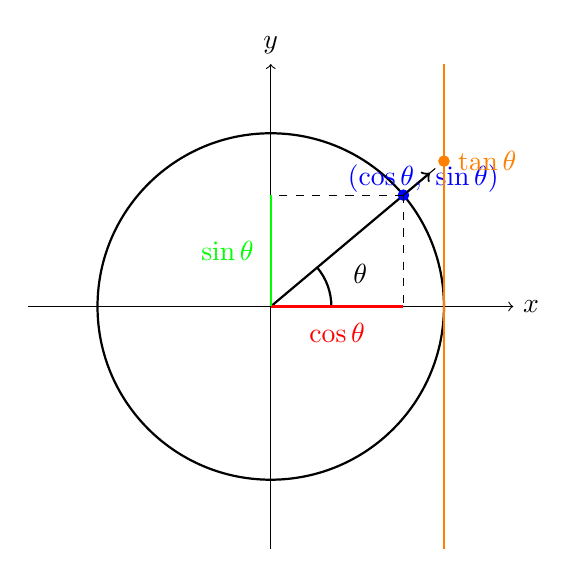
\begin{tikzpicture}[scale=2.2]
% Axes
\draw[->] (-1.4,0) -- (1.4,0) node[right] {$x$};
\draw[->] (0,-1.4) -- (0,1.4) node[above] {$y$};
% Unit circle
\draw[thick] (0,0) circle (1);
% Angle arc
\draw[thick] (0.35,0) arc (0:40:0.35);
% Angle label (near the origin)
\node at (20:0.55) {$\theta$};
% Ray forming the angle
\draw[thick,->] (0,0) -- (40:1.2);
% Point on the circle
\filldraw[blue] (40:1) circle (0.03);
\node[blue] at (40:1.15) {$(\cos\theta,\ \sin\theta)$};
% Cosine projection
\draw[dashed] (40:1) -- ({cos(40)},0);
\draw[thick,red] (0,0) -- ({cos(40)},0);
\node[red] at ({cos(40)/2},-0.15) {$\cos\theta$};
% Sine projection
\draw[dashed] (40:1) -- (0,{sin(40)});
\draw[thick,green] (0,0) -- (0,{sin(40)});
\node[green] at (-0.25,{sin(40)/2}) {$\sin\theta$};
% Tangent line
\draw[orange,thick] (1, -1.4) -- (1, 1.4);
\draw[dashed] (40:1) -- (1,{tan(40)});
\filldraw[orange] (1,{tan(40)}) circle (0.03);
\node[orange] at (1.25,{tan(40)}) {$\tan\theta$};
\end{tikzpicture} \end{center}
\subsection*{Interpretation}
\begin{itemize}
\item $\cos\theta$ is the horizontal coordinate of the point on the unit circle.
\item $\sin\theta$ is the vertical coordinate.
\item $\tan\theta$ is the length of the segment where the ray at angle $\theta$
intersects the vertical line $x=1$. \end{itemize}
Thus the trigonometric functions arise naturally from the geometry of the unit circle.
\subsection{Inverse functions}
A function may admit an inverse only when it is \emph{injective}: different inputs must produce different outputs.
Formally, a function $f : A \to B$ is injective when
\[ f(x_1)=f(x_2) \;\Rightarrow\; x_1=x_2. \]
Injectivity ensures that every value in the image of $f$ corresponds to exactly one input.
In this case one can define the \emph{inverse function} $f^{-1}$, which reverses the action of $f$.
\begin{definition}[Inverse function] Let $f : A \to B$ be an injective function.
The \emph{inverse function} of $f$ is the map
\[ f^{-1} : f(A) \to A \]
satisfying
\[ f^{-1}(f(x)) = x \qquad \text{for all } x\in A. \]
\end{definition}
The graph of $f^{-1}$ is obtained by reflecting the graph of $f$ across the line $y=x$, called the \emph{bisector} of the first and third quadrants.
\subsection*{Geometric representation}
\begin{center} 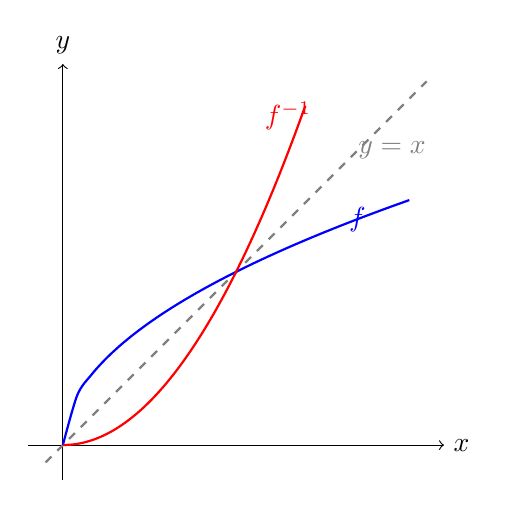
\begin{tikzpicture}[scale=2.2]
% Axes
\draw[->] (-0.2,0) -- (2.2,0) node[right] {$x$};
\draw[->] (0,-0.2) -- (0,2.2) node[above] {$y$};
% Bisector y = x
\draw[gray,thick,dashed] (-0.1,-0.1) -- (2.1,2.1);
\node[gray] at (1.9,1.7) {$y=x$};
% Function f(x) = sqrt(x)
\draw[blue,thick,domain=0:2,smooth,variable=\x]
plot ({\x},{sqrt(\x)});
\node[blue] at (1.7,1.3) {$f$};
% Inverse function f^{-1}(x) = x^2
\draw[red,thick,domain=0:1.4,smooth,variable=\x]
plot ({\x},{\x*\x});
\node[red] at (1.3,1.9) {$f^{-1}$};
\end{tikzpicture} \end{center}
The bisector $y=x$ shows that the inverse function is obtained by exchanging the roles of input and output: the graph of $f^{-1}$ is the reflection of the graph of $f$ across this line.
\section{Limits and continuity}
Many concepts in calculus are based on the idea of approaching a value without necessarily reaching it.
The simplest objects that illustrate this behaviour are \emph{sequences} of real numbers.
They provide the first setting in which limits are defined and studied.
\subsection{Sequences}
A \emph{sequence} is an ordered list of real numbers
\[ (a_n)_{n\ge 0} = a_0, a_1, a_2, \ldots \]
indexed by the integers $n\ge 0$.
Formally, a sequence is a function
\[ a : \mathbb{N} \to \mathbb{R}, \qquad n \mapsto a_n, \]
where $\mathbb{N}$ denotes the set of non’negative integers.
The value $a_n$ is called the \emph{$n$’th term} of the sequence.
A sequence may be described by an explicit formula (for example $a_n = 1/n$) or by a recurrence relation (for example $a_{n+1} = q\,a_n$).
\subsection{Convergence of a sequence}
A sequence may approach a real number as $n$ becomes large.
This behaviour is captured by the notion of \emph{limit}.
\begin{definition}[Limit of a sequence] A sequence $(a_n)$ \emph{converges} to a real number $L$ if for every $\varepsilon > 0$ there exists an integer $N$ such that
\[ |a_n - L| < \varepsilon \qquad \text{for all } n \ge N. \]
In this case one writes
\[ \lim_{n\to\infty} a_n = L. \]
\end{definition}
If no such real number $L$ exists, the sequence is said to \emph{diverge}.
\subsection{Eventual behaviour of a sequence}
Many properties of sequences do not need to hold for every index.
It is often enough that they hold \emph{eventually}, that is, from some point onward.
\begin{definition}[Eventually] Let $(a_n)$ be a sequence of real numbers.
A property $P(n)$ is said to hold \emph{eventually} (or \emph{for all sufficiently large $n$}) if there exists an integer $N$ such that
\[ P(n) \qquad \text{holds for all } n \ge N. \]
\end{definition}
In other words, a sequence may fail to satisfy $P(n)$ for the first few terms, but as long as the property holds for all indices beyond some threshold $N$, it is considered to hold eventually.
This notion is fundamental in limit theory, where statements about $a_n$ approaching a value concern the behaviour of the sequence for large $n$, not its initial terms.
\subsection{Types of behaviour of a sequence}
A sequence may exhibit different kinds of behaviour as the index $n$ becomes large.
The standard distinction is the following.
\subsubsection*{Convergent sequences}
A sequence $(a_n)$ is \emph{convergent} if it has a real limit, that is, if there exists $L\in\mathbb{R}$ such that
\[ \lim_{n\to\infty} a_n = L. \]
\subsubsection*{Sequences divergent to infinity}
A sequence is said to \emph{diverge to $+\infty$} if its terms grow without bound, meaning that for every $M\in\mathbb{R}$ there exists $N$ such that
\[ a_n > M \qquad \text{for all } n \ge N. \]
Similarly, it \emph{diverges to $-\infty$} if for every $M\in\mathbb{R}$ there exists $N$ such that
\[ a_n < M \qquad \text{for all } n \ge N. \]
In this sense, a “divergent sequence” is one whose terms tend to infinity in absolute value.
\subsubsection*{Sequences that are neither convergent nor divergent}
A sequence may fail to converge and also fail to diverge to $\pm\infty$.
Such sequences are described as \emph{neither convergent nor divergent}.
They may display oscillatory behaviour, irregular variation, or possess multiple accumulation points.
These sequences do not approach any single real value, nor do they grow without bound.
\subsection{Squeeze Theorem}
The Squeeze Theorem provides a useful criterion for determining the limit of a sequence by comparing it with two other sequences whose limits are known.
\begin{theorem}[Squeeze Theorem] Let $(a_n)$, $(b_n)$, and $(c_n)$ be sequences of real numbers such that
\[ a_n \le b_n \le c_n \qquad \text{for all sufficiently large } n. \]
If
\[ \lim_{n\to\infty} a_n = L \qquad \text{and} \qquad \lim_{n\to\infty} c_n = L, \]
then the sequence $(b_n)$ also converges to $L$, that is,
\[ \lim_{n\to\infty} b_n = L. \]
\end{theorem}
The theorem states that if a sequence is eventually trapped between two convergent sequences sharing the same limit, then it must converge to that limit as well.
\subsection{The exponential limit and the number $e$}
The number $e$ plays a central role in calculus and analysis.
It is defined through the behaviour of a specific sequence.
\begin{theorem}[Limit defining the number $e$] The sequence
\[ a_n = \left(1+\frac{1}{n}\right)^n \]
is increasing and bounded above.
Therefore it is convergent, and its limit is denoted by $e$:
\[ \lim_{n\to\infty} \left(1+\frac{1}{n}\right)^n = e. \]
\end{theorem}
The number $e$ is thus characterized as the unique real value approached by the sequence $\left(1+\frac{1}{n}\right)^n$ as $n$ becomes large.
This limit provides the fundamental definition of the base of the natural logarithm.
\subsection{Asymptotic comparisons and estimates}
Asymptotic analysis studies the behaviour of sequences for large values of the index.
It provides tools to compare the growth of different sequences and to obtain useful approximations.
\subsection*{Asymptotic comparison}
Let $(a_n)$ and $(b_n)$ be sequences of real numbers.
We say that $a_n$ and $b_n$ have the same asymptotic behaviour if
\[ \lim_{n\to\infty} \frac{a_n}{b_n} = 1. \]
In this case we write
\[ a_n \sim b_n, \]
and say that $a_n$ is \emph{asymptotically equivalent} to $b_n$.
This relation expresses that the two sequences grow at the same rate, even if their initial terms may differ.
\subsection*{Asymptotic estimates}
A sequence $(a_n)$ is said to be \emph{of smaller order} than $(b_n)$ if
\[ \lim_{n\to\infty} \frac{a_n}{b_n} = 0, \]
and we write
\[ a_n = o(b_n). \]
This means that $a_n$ grows strictly slower than $b_n$.
Similarly, we say that $a_n$ is \emph{bounded in order} by $b_n$ if there exists a constant $C>0$ such that
\[ |a_n| \le C\,|b_n| \qquad \text{for all sufficiently large } n. \]
In this case we write
\[ a_n = O(b_n). \]
These notations allow us to express growth rates and approximations in a concise and effective way.
\subsection*{Asymptotic inequalities}
Asymptotic comparisons often rely on inequalities that hold eventually.
If for sufficiently large $n$ we have
\[ a_n \le b_n, \]
then the growth of $(a_n)$ is asymptotically controlled by that of $(b_n)$. Such inequalities are frequently used to establish limits or to derive asymptotic estimates.
\subsection{Ratio Test}
The ratio test provides a useful criterion for determining whether a sequence diverges to $+\infty$ or converges to $0$, based on the behaviour of the ratio between consecutive terms.
\begin{theorem}[Ratio Test] Let $(a_n)$ be a sequence of positive real numbers and suppose that the limit
\[ L = \lim_{n\to\infty} \frac{a_{n+1}}{a_n} \]
exists.
\begin{itemize}
\item If $L < 1$, then the sequence $(a_n)$ converges to $0$.
\item If $L > 1$, then the sequence $(a_n)$ diverges to $+\infty$.
\item If $L = 1$, the test is inconclusive: the sequence may converge, diverge,
or display irregular behaviour. \end{itemize} \end{theorem}
The ratio test compares the growth of consecutive terms.
If each term is eventually smaller than the previous one by a fixed proportion, the sequence must tend to zero.
If each term is eventually larger by a fixed proportion, the sequence grows without bound.
\subsection{Uniqueness of the limit}
The limit of a sequence, when it exists, is uniquely determined.
This fundamental property ensures that a sequence cannot converge to two different real numbers.
\begin{theorem}[Uniqueness of the limit] Let $(a_n)$ be a sequence of real numbers.
If $(a_n)$ converges to $L$ and also converges to $M$, then
\[ L = M. \]
\end{theorem}
In other words, a convergent sequence cannot have two distinct limits.
The eventual behaviour of the sequence determines a single real value, which is its unique limit.
\subsection{Right and left limits of a function}
When studying the behaviour of a function near a point, it is often necessary to distinguish between approaching the point from the left or from the right.
\begin{definition}[Right limit] Let $f$ be a real function and let $x_0$ be a point in its domain.
The \emph{right limit} of $f$ at $x_0$ is the value $L$ such that
\[ \lim_{x \to x_0^+} f(x) = L, \]
meaning that $f(x)$ approaches $L$ as $x$ approaches $x_0$ from values greater than $x_0$. \end{definition}
\begin{definition}[Left limit] The \emph{left limit} of $f$ at $x_0$ is the value $M$ such that
\[ \lim_{x \to x_0^-} f(x) = M, \]
meaning that $f(x)$ approaches $M$ as $x$ approaches $x_0$ from values smaller than $x_0$. \end{definition}
\subsection*{Existence of the limit}
A function has a limit at a point if and only if both one-sided limits exist and are equal.
\begin{theorem}[Existence of the limit] Let $f$ be a real function and let $x_0$ be a point in its domain.
The limit
\[ \lim_{x \to x_0} f(x) \]
exists and equals $L$ if and only if
\[ \lim_{x \to x_0^-} f(x) = L \qquad \text{and} \qquad \lim_{x \to x_0^+} f(x) = L. \]
\end{theorem}
Thus, the behaviour of the function near $x_0$ is fully determined by its left-hand and right-hand limits.
If these two values coincide, the function has a well-defined limit at $x_0$.
\subsection*{Jump discontinuity}
A function may fail to be continuous at a point because its left-hand and right-hand limits exist but are different.
This type of discontinuity is called a \emph{jump discontinuity}.
\begin{definition}[Jump discontinuity] Let $f$ be a real function and let $x_0$ be a point in its domain.
We say that $f$ has a \emph{jump discontinuity} at $x_0$ if the one-sided limits
\[ \lim_{x \to x_0^-} f(x) \qquad \text{and} \qquad \lim_{x \to x_0^+} f(x) \]
both exist as finite real numbers, but
\[ \lim_{x \to x_0^-} f(x) \ne \lim_{x \to x_0^+} f(x). \]
\end{definition}
In this case the function “jumps” from one value to another when crossing the point $x_0$.
The function cannot be continuous at $x_0$, since continuity requires the left-hand and right-hand limits to coincide and equal the value of the function.
\subsection{Neighbourhood of a point}
The behaviour of a function near a point is often described using the notion of a neighbourhood.
A neighbourhood specifies a small interval around a point, without necessarily including the point itself.
\begin{definition}[Neighbourhood] Let $x_0 \in \mathbb{R}$ and let $\delta > 0$.
The \emph{neighbourhood} of $x_0$ of radius $\delta$ is the interval
\[ (x_0 - \delta,\; x_0 + \delta). \]
It contains all real numbers whose distance from $x_0$ is less than $\delta$. \end{definition}
\begin{definition}[Punctured neighbourhood] The \emph{punctured neighbourhood} of $x_0$ of radius $\delta$ is the set
\[ (x_0 - \delta,\; x_0 + \delta) \setminus \{x_0\}. \]
It includes all points sufficiently close to $x_0$, but excludes $x_0$ itself. \end{definition}
Neighbourhoods and punctured neighbourhoods are used to describe limits and continuity, since limits concern the behaviour of a function near a point rather than at the point itself.
\subsection{Change of variable in limits}
When evaluating limits, it is often useful to replace the variable with another expression that approaches the same value.
The following theorem formalizes this idea.
\begin{theorem}[Change of variable in limits] Let $f$ be a real function and let $g$ be another function such that
\[ \lim_{x \to x_0} g(x) = L. \]
If the limit
\[ \lim_{y \to L} f(y) \]
exists and equals $M$, then the composite limit
\[ \lim_{x \to x_0} f(g(x)) \]
also exists and equals $M$. \end{theorem}
In other words, if $g(x)$ approaches $L$ as $x$ approaches $x_0$, and $f(y)$ approaches $M$ as $y$ approaches $L$, then the composition $f(g(x))$ approaches $M$ as $x$ approaches $x_0$.
The change of variable allows us to evaluate limits by substituting the inner expression with its limiting value.
\subsection{Continuity of elementary functions}
Elementary functions encountered in calculus possess strong continuity properties.
The following results summarize the fundamental facts.
\begin{definition}[Continuity of elementary functions] The basic elementary functions — polynomials, rational functions (where defined), exponential and logarithmic functions, trigonometric and inverse trigonometric functions — are continuous on every point of their domain. \end{definition}
\begin{definition}[Continuity preserved by algebraic operations] Let $f$ and $g$ be continuous at a point $x_0$.
Then the functions
\[ f+g,\qquad f-g,\qquad f\cdot g,\qquad \frac{f}{g}\ \text{(if } g(x_0)\ne 0) \]
are also continuous at $x_0$. \end{definition}
\begin{definition}[Continuity preserved by composition] If $f$ is continuous at $x_0$ and $g$ is continuous at $f(x_0)$, then the composition $g\circ f$ is continuous at $x_0$:
\[ \lim_{x\to x_0} g(f(x)) = g\bigl(\lim_{x\to x_0} f(x)\bigr). \]
\end{definition}
These properties ensure that any function built from elementary functions using algebraic operations and composition remains continuous on its domain.
\subsection{Fundamental limits}
Certain limits play a central role in calculus and appear frequently in the study of derivatives, continuity, and asymptotic behaviour.
These are known as \emph{fundamental limits}.
\begin{itemize}
\item \textbf{Exponential limit}
\[
\lim_{x \to 0} (1+x)^{1/x} = e.
\]
\item \textbf{Logarithmic limit}
\[
\lim_{x \to 0} \frac{\ln(1+x)}{x} = 1.
\]
\item \textbf{Trigonometric limits}
\[
\lim_{x \to 0} \frac{\sin x}{x} = 1,
\qquad
\lim_{x \to 0} \frac{1 - \cos x}{x^2} = \frac{1}{2}.
\]
\item \textbf{Exponential growth limit}
\[
\lim_{x \to 0} \frac{e^x - 1}{x} = 1.
\]
\item \textbf{Power limit}
\[
\lim_{x \to 0} \frac{x^n}{x} = 0 \qquad \text{for every } n>1.
\]
\end{itemize}
These limits are used to compute derivatives of elementary functions and to establish many foundational results in analysis.
They also serve as reference points for approximations and asymptotic estimates.
\subsection{Theorem of the zeros}
A continuous function on an interval cannot change sign without crossing the value zero.
This fundamental result is known as the \emph{Theorem of the zeros}.
\begin{theorem}[Theorem of the zeros] Let $f$ be a real function that is continuous on the closed interval $[a,b]$. If
\[ f(a)\cdot f(b) < 0, \]
that is, if $f(a)$ and $f(b)$ have opposite signs, then there exists at least one point $c \in (a,b)$ such that
\[ f(c) = 0. \]
\end{theorem}
In other words, a continuous function that takes positive values at one endpoint of an interval and negative values at the other must vanish somewhere inside the interval.
The function cannot “jump over” the value zero without violating continuity.
\subsection{Weierstrass Theorem}
A continuous function defined on a closed and bounded interval always reaches its largest and smallest values.
This fundamental result is known as the \emph{Weierstrass Theorem}.
\begin{theorem}[Weierstrass Theorem] Let $f$ be a real function that is continuous on the closed interval $[a,b]$. Then $f$ is bounded on $[a,b]$, and there exist points
\[ x_{\min},\; x_{\max} \in [a,b] \]
such that
\[ f(x_{\min}) = \min_{x \in [a,b]} f(x), \qquad f(x_{\max}) = \max_{x \in [a,b]} f(x). \]
\end{theorem}
In other words, a continuous function on a closed interval cannot “escape” to infinity and cannot approach its extrema without attaining them.
The compactness of the interval ensures both boundedness and the existence of maximum and minimum values.
\subsection{Intermediate Value Theorem}
A continuous function on an interval cannot “skip” values.
If it takes two different values at the endpoints of an interval, then it must take every value in between.
This fundamental result is known as the \emph{Intermediate Value Theorem}.
\begin{theorem}[Intermediate Value Theorem] Let $f$ be a real function that is continuous on the closed interval $[a,b]$. Let $L$ be any real number between $f(a)$ and $f(b)$, that is,
\[ f(a) < L < f(b) \quad \text{or} \quad f(b) < L < f(a). \]
Then there exists at least one point $c \in (a,b)$ such that
\[ f(c) = L. \]
\end{theorem}
In other words, a continuous function on an interval takes all intermediate values between its values at the endpoints.
The function cannot jump over any value without violating continuity.
\subsection{Existence and uniqueness of the $n$th root}
The $n$th root of a positive real number is well defined and unique.
This fundamental property ensures that the equation $x^n = y$ has exactly one positive solution.
\begin{theorem}[Existence and uniqueness of the $n$th root] For every real number $y>0$ and every integer $n \ge 1$, there exists one and only one real number $x>0$ such that
\[ x^n = y. \]
This number is called the $n$th root of $y$ and is denoted by $\sqrt[n]{y}$. \end{theorem}
In other words, the function $x \mapsto x^n$ is continuous and strictly increasing on $(0,+\infty)$, and therefore it admits a unique inverse on this interval.
This inverse function assigns to each positive $y$ its unique positive $n$th root.
\subsection{Monotonicity theorem for functions}
A monotone function on an interval has well’defined one’sided limits at every point of the interval.
Inside the interval these limits are finite, while at the endpoints they may be finite or infinite.
\begin{theorem}[Monotonicity theorem] Let $f$ be a real function that is monotone (increasing or decreasing) on the interval $[a,b]$.
\begin{itemize}
\item For every point $x_0 \in (a,b)$, both one’sided limits
\[
\lim_{x \to x_0^-} f(x)
\qquad\text{and}\qquad
\lim_{x \to x_0^+} f(x)
\]
exist and are finite.
\item At the left endpoint $a$, the right’hand limit
\[
\lim_{x \to a^+} f(x)
\]
exists and may be finite or $+\infty$ or $-\infty$.
\item At the right endpoint $b$, the left’hand limit
\[
\lim_{x \to b^-} f(x)
\]
exists and may be finite or $+\infty$ or $-\infty$. \end{itemize} \end{theorem}
In other words, monotonicity ensures that the function has a well’defined behaviour near every point of the interval:
inside the interval the function cannot oscillate, and at the endpoints it may diverge but never oscillate.
\section{Differential Calculus}
Differential calculus studies how functions change and how their behaviour can be described locally.
Its central concept is the derivative, which measures the instantaneous rate of variation of a function with respect to its variable.
Through limits, we develop tools to understand linear approximations, tangent lines, and the sensitivity of functions to small changes in input.
This section introduces the derivative, explores its fundamental properties, and presents the main rules of differentiation.
We also examine differentiability, the relationship between continuity and derivatives, and the applications of derivatives to monotonicity, extrema, and the qualitative analysis of functions.
\subsection {Derivative of a function}
Let $f$ be a real function defined on a subset of $\mathbb{R}$.
As stated earlier, a function is a rule $f:A\to B$ that assigns to every $x\in A$ a unique real number $f(x)\in B$.
The derivative describes how $f(x)$ changes when $x$ varies.
\begin{definition}[Derivative] The \emph{derivative} of $f$ at a point $x_0$ is the limit
\[ f'(x_0) = \lim_{h\to 0} \frac{f(x_0+h)-f(x_0)}{h}, \]
if this limit exists. \end{definition}
The quotient
\[ \frac{f(x_0+h)-f(x_0)}{h} \]
is the slope of the secant line through the points $(x_0,f(x_0))$ and $(x_0+h,f(x_0+h))$.
The derivative $f'(x_0)$ is the slope of the tangent line obtained as the limit of these secant slopes.
\subsection {Slope and tangent line}
The tangent line to the graph of $f$ at $x_0$ is the line
\[ y = f(x_0) + f'(x_0)(x - x_0). \]
\begin{itemize}
\item If $f'(x_0)>0$, the graph is increasing at $x_0$.
\item If $f'(x_0)<0$, the graph is decreasing at $x_0$.
\item If $f'(x_0)=0$, the tangent line is horizontal. \end{itemize}
\subsection*{Angle of inclination}
Every nonvertical line has an angle of inclination $\theta$ with the positive $x$-axis.
The slope $m$ and the angle $\theta$ are related by
\[ m = \tan\theta. \]
Therefore, if the tangent line at $x_0$ makes an angle $\theta$ with the $x$-axis, then
\[ f'(x_0) = \tan\theta. \]
A large absolute value of $f'(x_0)$ corresponds to a steep tangent line.
If the tangent line is vertical, the angle is $\theta=\frac{\pi}{2}$ and the slope is undefined: the derivative does not exist at that point.
\subsection*{Elementary derivatives}
The following table collects the basic derivatives of the standard elementary functions.
Each formula holds for every $x$ in the domain where the expression is defined.
\begin{center} \renewcommand{\arraystretch}{1.4} \begin{tabular}{|c|c|} \hline \textbf{Function $f(x)$} & \textbf{Derivative $f'(x)$} \\ \hline $c$ (constant) & $0$ \\ \hline $x$ & $1$ \\ \hline $x^n$ (for $n\in\mathbb{Z}$) & $n x^{\,n-1}$ \\ \hline $\sqrt{x}$ & $\dfrac{1}{2\sqrt{x}}$ \\ \hline $\dfrac{1}{x}$ & $-\dfrac{1}{x^2}$ \\ \hline $\sin x$ & $\cos x$ \\ \hline $\cos x$ & $-\sin x$ \\ \hline $\tan x$ & $\sec^2 x$ \\ \hline $\cot x$ & $-\csc^2 x$ \\ \hline $\sec x$ & $\sec x \tan x$ \\ \hline $\csc x$ & $-\csc x \cot x$ \\ \hline $e^x$ & $e^x$ \\ \hline $a^x$ ($a>0$) & $a^x \ln a$ \\ \hline $\ln x$ & $\dfrac{1}{x}$ \\ \hline $\log_a x$ ($a>0$) & $\dfrac{1}{x \ln a}$ \\ \hline \end{tabular} \end{center}
\subsection {Corner points, cusps, and inflection points}
The derivative describes the local behaviour of the graph of a function.
Certain characteristic points occur when the derivative fails to exist or when the curvature of the graph changes.
\subsection*{Corner point}
A point $x_0$ is a \emph{corner point} of the graph of $f$ if the one-sided derivatives
\[ f'_-(x_0) = \lim_{h\to 0^-} \frac{f(x_0+h)-f(x_0)}{h}, \qquad f'_+(x_0) = \lim_{h\to 0^+} \frac{f(x_0+h)-f(x_0)}{h} \]
both exist but are different:
\[ f'_-(x_0) \neq f'_+(x_0). \]
The tangent line has a sudden change of slope, producing a sharp angle on the graph.
\subsection*{Cusp}
A point $x_0$ is a \emph{cusp} if the one-sided derivatives diverge with opposite signs:
\[ f'_-(x_0) = -\infty, \qquad f'_+(x_0) = +\infty, \]
or vice versa.
The graph approaches a vertical tangent from both sides, but with incompatible directions, creating a pointed tip.
\subsection*{Inflection point}
A point $x_0$ is an \emph{inflection point} of $f$ if the function is differentiable near $x_0$ and the concavity changes sign.
Equivalently, the second derivative (when it exists) satisfies
\[ f''(x) < 0 \text{ for } x < x_0, \qquad f''(x) > 0 \text{ for } x > x_0, \]
or the opposite.
At an inflection point the tangent line exists and crosses the graph, marking the transition between concave and convex behaviour.
\subsection*{Summary}
\begin{itemize}
\item Corner point: one-sided derivatives exist but are different.
\item Cusp: one-sided derivatives diverge with opposite signs.
\item Inflection point: concavity changes sign; the tangent line exists. \end{itemize}
\subsection*{Continuity and differentiability}
Differentiability is a stronger property than continuity.
A function may be continuous without being differentiable, but every differentiable function is necessarily continuous.
\begin{theorem}[Differentiability implies continuity] Let $f$ be a function defined on an interval and let $x_0$ be a point in its domain.
If $f$ is differentiable at $x_0$, then $f$ is continuous at $x_0$. \end{theorem}
\begin{proof} If $f$ is differentiable at $x_0$, the limit
\[ f'(x_0)=\lim_{h\to 0}\frac{f(x_0+h)-f(x_0)}{h} \]
exists and is finite.
Multiplying both sides by $h$ gives
\[ f(x_0+h)-f(x_0)=h\,f'(x_0)+o(h), \]
where $o(h)\to 0$ as $h\to 0$.
Therefore,
\[ \lim_{h\to 0}\bigl(f(x_0+h)-f(x_0)\bigr)=0, \]
which is exactly the definition of continuity at $x_0$. \end{proof}
\subsection*{Continuity without differentiability}
The converse is false: continuity does not imply differentiability.
A function may be continuous at a point but fail to have a derivative there.
Typical examples include: \begin{itemize}
\item corner points (e.g.\ $f(x)=|x|$ at $x=0$),
\item cusps (e.g.\ $f(x)=x^{2/3}$ at $x=0$),
\item vertical tangents (e.g.\ $f(x)=\sqrt[3]{x}$ at $x=0$). \end{itemize}
\subsection*{Summary}
\begin{itemize}
\item Differentiability $\Rightarrow$ continuity.
\item Continuity $\not\Rightarrow$ differentiability.
\item Non-differentiability may occur at corners, cusps, or vertical tangents. \end{itemize}
\subsection {Derivative of an inverse function}
Let $f$ be a real function defined on an interval.
When $f$ is strictly monotonic, it is invertible, and its inverse function $f^{-1}$ is also defined on an interval.
The derivative of the inverse is determined by the derivative of $f$.
\begin{theorem}[Derivative of the inverse function] Let $f$ be a continuous and strictly monotonic function on an interval, and assume that $f$ is differentiable at a point $x_0$ with
\[ f'(x_0) \neq 0. \]
Then the inverse function $f^{-1}$ is differentiable at $y_0 = f(x_0)$, and its derivative is
\[ (f^{-1})'(y_0) = \frac{1}{f'(x_0)}. \]
Equivalently, for every $x$ in the domain of $f$,
\[ (f^{-1})'(f(x)) = \frac{1}{f'(x)}. \]
\end{theorem}
\begin{proof} Since $f$ is strictly monotonic, it admits an inverse $f^{-1}$.
For $y$ near $y_0=f(x_0)$, write $y=f(x)$, so that $x=f^{-1}(y)$.
Then
\[ \frac{f^{-1}(y)-f^{-1}(y_0)}{y-y_0} = \frac{x-x_0}{f(x)-f(x_0)}. \]
Taking the limit as $y\to y_0$ (equivalently $x\to x_0$) gives
\[ (f^{-1})'(y_0) = \lim_{x\to x_0} \frac{x-x_0}{f(x)-f(x_0)} = \frac{1}{f'(x_0)}. \]
\end{proof}
\subsection*{Interpretation}
The derivative of the inverse function is the reciprocal of the derivative of the original function.
Geometrically, the graph of $f^{-1}$ is the reflection of the graph of $f$ across the line $y=x$, and the slope transforms by inversion:
\[ m_{f^{-1}} = \frac{1}{m_f}. \]
\subsection*{Example}
For $f(x)=e^x$, the inverse is $f^{-1}(y)=\ln y$.
Since $f'(x)=e^x$, we obtain
\[ (\ln y)' = \frac{1}{y}, \]
in agreement with the theorem.
\subsection {Fermat's theorem}
Critical points of a function occur where the derivative is zero or does not exist.
Fermat's theorem gives a necessary condition for a local extremum when the derivative exists.
\begin{theorem}[Fermat's theorem] Let $f$ be a real function defined on an interval, and let $x_0$ be an interior point of the interval.
If $f$ has a local maximum or a local minimum at $x_0$ and $f$ is differentiable at $x_0$, then
\[ f'(x_0) = 0. \]
\end{theorem}
\begin{proof} Assume $f$ has a local maximum at $x_0$.
Then there exists a neighbourhood of $x_0$ such that
\[ f(x) \le f(x_0) \qquad \text{for all } x \text{ near } x_0. \]
For $h>0$ small,
\[ \frac{f(x_0+h)-f(x_0)}{h} \le 0, \]
and for $h<0$ small,
\[ \frac{f(x_0+h)-f(x_0)}{h} \ge 0. \]
Taking the limits as $h\to 0^+$ and $h\to 0^-$ shows that the right and left derivatives exist and are both equal to $0$.
Thus $f'(x_0)=0$.
The case of a local minimum is analogous. \end{proof}
\subsection*{Consequences}
\begin{itemize}
\item If $f'(x_0)\neq 0$, then $f$ cannot have a local extremum at $x_0$.
\item If $f'(x_0)=0$, the point $x_0$ is a \emph{critical point}, but it may be:
\begin{itemize}
\item a local maximum,
\item a local minimum,
\item or neither (e.g.\ an inflection point).
\end{itemize}
\item If $f$ is not differentiable at $x_0$, a local extremum may still occur (e.g.\ $f(x)=|x|$ at $x=0$). \end{itemize}
\subsection*{Example}
For $f(x)=x^3$, we have $f'(x)=3x^2$, so $f'(0)=0$.
However, $x=0$ is not a local extremum: the function is increasing on both sides.
This illustrates that $f'(x_0)=0$ is a necessary but not sufficient condition for an extremum.
\subsection {Mean Value Theorem (Lagrange's theorem)}
The Mean Value Theorem is one of the fundamental results of differential calculus.
It states that for every sufficiently regular function, there exists a point where the instantaneous rate of change equals the average rate of change over an interval.
\begin{theorem}[Mean Value Theorem] Let $f$ be a real function that is continuous on the closed interval $[a,b]$ and differentiable on the open interval $(a,b)$, with $a<b$.
Then there exists at least one point $c\in(a,b)$ such that
\[ f'(c) = \frac{f(b)-f(a)}{b-a}. \]
\end{theorem}
\begin{proof} Define the auxiliary function
\[ g(x) = f(x) - \left( f(a) + \frac{f(b)-f(a)}{b-a}(x-a) \right). \]
The function $g$ is continuous on $[a,b]$ and differentiable on $(a,b)$, and satisfies $g(a)=g(b)=0$.
By Rolle's theorem, there exists $c\in(a,b)$ such that $g'(c)=0$.
Computing the derivative,
\[ g'(x) = f'(x) - \frac{f(b)-f(a)}{b-a}, \]
so $g'(c)=0$ implies
\[ f'(c) = \frac{f(b)-f(a)}{b-a}. \]
\end{proof}
\subsection*{Interpretation}
The quantity
\[ \frac{f(b)-f(a)}{b-a} \]
is the slope of the secant line joining the points $(a,f(a))$ and $(b,f(b))$.
The theorem guarantees that somewhere between $a$ and $b$, the tangent line has exactly the same slope.
Thus the instantaneous rate of change equals the average rate of change at some point.
\subsection*{Consequences}
\begin{itemize}
\item If $f'(x)=0$ for all $x\in(a,b)$, then $f$ is constant on $[a,b]$.
\item If $f'(x)>0$ for all $x\in(a,b)$, then $f$ is strictly increasing on $[a,b]$.
\item If $f'(x)<0$ for all $x\in(a,b)$, then $f$ is strictly decreasing on $[a,b]$. \end{itemize}
\subsection*{Example}
For $f(x)=x^2$ on $[1,3]$, the average rate of change is
\[ \frac{f(3)-f(1)}{3-1} = \frac{9-1}{2} = 4. \]
Since $f'(x)=2x$, the equation $2c=4$ gives $c=2$, which lies in $(1,3)$, as guaranteed by the theorem.
\subsection {Monotonicity test}
The derivative provides a precise criterion to determine whether a function is increasing or decreasing on an interval.
This result is known as the \emph{monotonicity test}.
\begin{theorem}[Monotonicity test] Let $f$ be a real function that is continuous on a closed interval $[a,b]$ and differentiable on the open interval $(a,b)$. \begin{itemize}
\item If $f'(x) > 0$ for all $x \in (a,b)$, then $f$ is strictly increasing on $[a,b]$.
\item If $f'(x) < 0$ for all $x \in (a,b)$, then $f$ is strictly decreasing on $[a,b]$.
\item If $f'(x) = 0$ for all $x \in (a,b)$, then $f$ is constant on $[a,b]$. \end{itemize} \end{theorem}
\begin{proof} Assume $f'(x) > 0$ for all $x \in (a,b)$.
For any $x_1, x_2 \in (a,b)$ with $x_1 < x_2$, the Mean Value Theorem gives a point $c \in (x_1, x_2)$ such that
\[ f'(c) = \frac{f(x_2) - f(x_1)}{x_2 - x_1}. \]
Since $f'(c) > 0$ and $x_2 - x_1 > 0$, we obtain $f(x_2) > f(x_1)$, proving that $f$ is strictly increasing.
The decreasing and constant cases follow analogously. \end{proof}
\subsection*{Interpretation}
The sign of the derivative determines the behaviour of the function: \begin{itemize}
\item Positive derivative $\Rightarrow$ the function rises.
\item Negative derivative $\Rightarrow$ the function falls.
\item Zero derivative $\Rightarrow$ the function is flat (constant). \end{itemize}
\subsection*{Example}
For $f(x)=x^3$, we have $f'(x)=3x^2 \ge 0$ for all $x$.
The derivative is never negative, and equals $0$ only at $x=0$.
Thus $f$ is increasing on every interval, even though the slope is horizontal at the origin.
\subsection {L'Hospital's rule}
L'Hospital's rule is a fundamental tool for evaluating limits that produce indeterminate forms of type $\frac{0}{0}$ or $\frac{\infty}{\infty}$.
\begin{theorem}[L'Hospital's rule] Let $f$ and $g$ be real functions differentiable on an open interval $(a,b)$, and suppose that
\[ \lim_{x\to c} f(x) = 0, \qquad \lim_{x\to c} g(x) = 0, \]
or
\[ \lim_{x\to c} f(x) = \pm\infty, \qquad \lim_{x\to c} g(x) = \pm\infty, \]
for some point $c\in(a,b)$ (or $c$ equal to an endpoint).
Assume also that $g'(x)\neq 0$ for all $x$ near $c$, and that the limit
\[ \lim_{x\to c} \frac{f'(x)}{g'(x)} \]
exists (finite or infinite).
Then
\[ \lim_{x\to c} \frac{f(x)}{g(x)} = \lim_{x\to c} \frac{f'(x)}{g'(x)}. \]
\end{theorem}
\subsection*{Interpretation}
When the quotient $\frac{f(x)}{g(x)}$ produces an indeterminate form $\frac{0}{0}$ or $\frac{\infty}{\infty}$, the limit can be computed by differentiating the numerator and denominator separately.
The rule does not apply to other indeterminate forms such as $0\cdot\infty$, $\infty-\infty$, $1^\infty$, $0^0$, or $\infty^0$ without additional transformations.
\subsection*{Example}
Consider the limit
\[ \lim_{x\to 0} \frac{\sin x}{x}. \]
Both numerator and denominator tend to $0$, so the form is $\frac{0}{0}$.
Applying L'Hospital's rule,
\[ \lim_{x\to 0} \frac{\sin x}{x} = \lim_{x\to 0} \frac{\cos x}{1} = 1. \]
\subsection*{Another example}
For
\[ \lim_{x\to +\infty} \frac{e^x}{x^3}, \]
both numerator and denominator tend to $+\infty$.
Applying L'Hospital's rule repeatedly,
\[ \frac{e^x}{x^3} \;\longrightarrow\; \frac{e^x}{3x^2} \;\longrightarrow\; \frac{e^x}{6x} \;\longrightarrow\; \frac{e^x}{6}, \]
so the limit is $+\infty$.
\subsection {Limit of the derivative and one-sided differentiability}
The behaviour of the derivative near an endpoint determines whether the one-sided derivative exists at that endpoint.
\begin{theorem}[One-sided derivative from the limit of the derivative] Let $f$ be a real function defined on the interval $[a,b)$, with $b$ possibly $+\infty$.
Assume that: \begin{itemize}
\item $f$ is continuous at $a$;
\item $f$ is differentiable on $(a,b)$;
\item the limit
\[
\lim_{x\to a^+} f'(x) = m
\]
exists, finite or infinite. \end{itemize} Then the right-hand derivative of $f$ at $a$ exists and satisfies
\[ f'_+(a) = m. \]
\end{theorem}
\subsection*{Left-hand version}
If $f$ is defined on $(a,b]$, continuous at $b$, differentiable on $(a,b)$, and
\[ \lim_{x\to b^-} f'(x) = m, \]
then the left-hand derivative at $b$ exists and equals $m$:
\[ f'_-(b) = m. \]
\subsection {Second derivative}
The second derivative describes how the rate of change of a function varies.
While the first derivative measures the slope of the tangent line, the second derivative measures the curvature of the graph.
\begin{definition}[Second derivative] Let $f$ be a differentiable function on an interval.
If the derivative $f'$ is differentiable, the \emph{second derivative} of $f$ is
\[ f''(x) = (f'(x))'. \]
\end{definition}
\subsection*{Geometric meaning}
The second derivative indicates how the graph bends:
\begin{itemize}
\item If $f''(x) > 0$, the graph is \emph{concave up}: the tangent slope is increasing, and the curve bends upward like a cup.
\item If $f''(x) < 0$, the graph is \emph{concave down}: the tangent slope is decreasing, and the curve bends downward like an arch.
\item If $f''(x_0) = 0$, the point $x_0$ may be an \emph{inflection point}, where the concavity changes sign. \end{itemize}
Thus the second derivative provides information about the shape of the graph and helps identify inflection points and classify critical points.
\subsection {Continuity of convex and concave functions}
Convexity and concavity impose strong regularity conditions on a function.
In particular, a convex or concave function cannot have interior discontinuities.
\begin{theorem}[Continuity of convex and concave functions] Let $f$ be a real function defined on an interval $I$ (open, closed, or half-open).
If $f$ is convex or concave on $I$, then $f$ is continuous at every interior point of $I$.
Possible discontinuities may occur only at the endpoints of $I$. \end{theorem}
\subsection*{Interpretation}
A convex or concave function cannot “jump” inside the interval:
its graph must bend smoothly without breaks.
However, if the interval has endpoints (for example $[a,b)$ or $(a,b]$), the function may fail to be continuous at $a$ or $b$, but never in the interior.
Convexity and concavity therefore guarantee: \begin{itemize}
\item continuity on the interior of the interval;
\item no oscillations or jumps inside the interval;
\item possible discontinuities only at the boundary points. \end{itemize}
\subsection {Convexity and derivatives}
Convexity can be characterized through the behaviour of the derivative.
A convex function has a non’decreasing derivative; a concave function has a non’increasing derivative.
\begin{theorem}[Convexity and derivatives] Let $f$ be a real function defined on an interval $I$ and differentiable on the interior of $I$. \begin{itemize}
\item $f$ is convex on $I$ if and only if its derivative $f'$ is non-decreasing on $I$.
\item $f$ is concave on $I$ if and only if its derivative $f'$ is non-increasing on $I$. \end{itemize} If $f$ is twice differentiable, these conditions are equivalent to: \begin{itemize}
\item $f''(x) \ge 0$ for all $x$ in $I$
\quad (convexity),
\item $f''(x) \le 0$ for all $x$ in $I$
\quad (concavity). \end{itemize} \end{theorem}
\subsection*{Geometric meaning}
\begin{itemize}
\item For a convex function, the slope of the tangent line increases: the graph bends upward.
\item For a concave function, the slope of the tangent line decreases: the graph bends downward.
\item The sign of the second derivative describes the curvature of the graph. \end{itemize}
Convexity therefore corresponds to “accelerating slope”, while concavity corresponds to “decelerating slope”.
\subsection {Convexity and tangent lines}
Convexity has a clear geometric interpretation in terms of tangent lines.
For a convex function, every tangent line lies below the graph; for a concave function, every tangent line lies above it.
\begin{theorem}[Convexity and tangent lines] Let $f$ be a real function defined on an interval $I$ and differentiable on the interior of $I$. \begin{itemize}
\item If $f$ is convex on $I$, then for every $x_0 \in I$ and every $x \in I$,
\[
f(x) \ge f(x_0) + f'(x_0)(x - x_0).
\]
That is, the tangent line at $x_0$ lies below the graph of $f$.
\item If $f$ is concave on $I$, then for every $x_0 \in I$ and every $x \in I$,
\[
f(x) \le f(x_0) + f'(x_0)(x - x_0).
\]
That is, the tangent line at $x_0$ lies above the graph of $f$. \end{itemize} \end{theorem}
\subsection*{Geometric meaning}
For a convex function: \begin{itemize}
\item the graph bends upward;
\item the slope of the tangent line increases;
\item every tangent line touches the graph from below. \end{itemize}
For a concave function: \begin{itemize}
\item the graph bends downward;
\item the slope of the tangent line decreases;
\item every tangent line touches the graph from above. \end{itemize}
This property is fundamental in optimization and in the geometric interpretation of convexity.
\subsection {Inflection points and the second derivative}
An inflection point is a point where the graph of a function changes concavity.
The second derivative provides a useful criterion for detecting such points.
\begin{theorem}[Inflection point and second derivative] Let $f$ be a real function defined on an interval and twice differentiable on the interior of the interval.
If $x_0$ is an inflection point of $f$, then the concavity changes sign at $x_0$, and therefore
\[ f''(x_0) = 0 \]
or the second derivative does not exist at $x_0$.
Conversely, if $f''(x_0)=0$ and the second derivative changes sign when passing through $x_0$, then $x_0$ is an inflection point of $f$. \end{theorem}
\subsection*{Geometric meaning}
At an inflection point: \begin{itemize}
\item the graph switches from concave up to concave down, or vice versa;
\item the tangent line exists and crosses the graph;
\item the second derivative typically vanishes, but this condition alone is not sufficient — the change of concavity is essential. \end{itemize}
Thus the second derivative helps identify inflection points, but the decisive criterion is the change in concavity.
\subsection {Inflection point and tangent line}
An inflection point is a point where the function changes concavity.
A key geometric property is that the tangent line at such a point intersects (or is crossed by) the graph.
\begin{theorem}[The tangent line at an inflection point] Let $f$ be a real function defined on an interval and differentiable at a point $x_0$.
If $x_0$ is an inflection point of $f$, then the tangent line at $x_0$
\[ T(x) = f(x_0) + f'(x_0)(x - x_0) \]
is crossed by the graph of $f$ at $x_0$.
Equivalently, the function lies on one side of the tangent line for $x < x_0$ and on the opposite side for $x > x_0$. \end{theorem}
\subsection*{Geometric meaning}
At an inflection point: \begin{itemize}
\item the concavity changes sign;
\item the tangent line touches the graph at $x_0$;
\item the graph passes from one side of the tangent to the other. \end{itemize}
Thus, the tangent line is not a supporting line (as in convex or concave functions), but a line that the curve actually crosses.
\subsection {Little-$o$ notation}
The little-$o$ notation describes a quantity that becomes negligible compared to another as the variable approaches a point.
It is used to express that one function goes to zero faster than another.
\begin{definition}[Little-$o$ notation] Let $g(x)$ be a nonzero function near a point $x_0$.
We say that
\[ f(x) = o\bigl(g(x)\bigr) \quad \text{as } x \to x_0 \]
if
\[ \lim_{x\to x_0} \frac{f(x)}{g(x)} = 0. \]
\end{definition}
\subsection*{Meaning}
The expression $f(x) = o(g(x))$ means that $f(x)$ becomes **small much faster** than $g(x)$ as $x$ approaches $x_0$.
Equivalently, $f(x)$ is negligible compared to $g(x)$ in that limit.
Typical examples: \begin{itemize}
\item $x = o(1)$ as $x\to 0$ (because $x/1 \to 0$),
\item $x^2 = o(x)$ as $x\to 0$ (because $x^2/x = x \to 0$),
\item $\sin x - x = o(x)$ as $x\to 0$. \end{itemize}
Little-$o$ notation is widely used in Taylor expansions and in expressing error terms.
\subsection*{Little-$o$ notation and linear approximation}
Little-$o$ notation is used to describe error terms that become negligible compared to a given quantity.
For a differentiable function, it provides a precise way to express the accuracy of the linear approximation.
\begin{definition}[Little-$o$ notation] We write
\[ f(x) = o(g(x)) \quad \text{as } x \to x_0 \]
if
\[ \lim_{x \to x_0} \frac{f(x)}{g(x)} = 0. \]
This means that $f(x)$ becomes negligible compared to $g(x)$ near $x_0$. \end{definition}
\subsection*{Usage in linear approximation}
If $f$ is differentiable at $x_0$, then for a small increment $dx$ we have the expansion
\[ f(x_0 + dx) = f(x_0) + f'(x_0)\,dx + o(dx) \quad \text{as } dx \to 0. \]
The term $o(dx)$ represents the error of the linear approximation: it is much smaller than $dx$ itself.
\subsection*{Differential}
The differential of $f$ at $x_0$ is defined as the linear part of the increment:
\[ df(x_0) = f'(x_0)\,dx. \]
Thus the change in the function can be written as
\[ f(x_0 + dx) - f(x_0) = df(x_0) + o(dx), \]
meaning that the differential gives the best linear approximation, and the little-$o$ term measures the deviation from linearity.
\subsection {Taylor--Maclaurin formula with Peano remainder}
The Taylor expansion expresses a function as a polynomial plus an error term that becomes negligible at small scales.
The Peano remainder gives a very compact way to describe this error.
\begin{theorem}[Taylor formula with Peano remainder] Let $f$ be a real function that is $n$ times differentiable at a point $x_0$.
Then, as $x \to x_0$,
\[ f(x) = f(x_0)
+ f'(x_0)(x - x_0)
+ \frac{f''(x_0)}{2!}(x - x_0)^2
+ \cdots
+ \frac{f^{(n)}(x_0)}{n!}(x - x_0)^n
+ o\!\left((x - x_0)^n\right). \]
If $x_0 = 0$, this becomes the Maclaurin expansion:
\[ f(x) = f(0)
+ f'(0)x
+ \frac{f''(0)}{2!}x^2
+ \cdots
+ \frac{f^{(n)}(0)}{n!}x^n
+ o(x^n)
\quad \text{as } x \to 0. \]
\end{theorem}
\subsection*{Meaning}
The term
\[ o\!\left((x - x_0)^n\right) \]
means that the remainder is **negligible compared to $(x - x_0)^n$** as $x$ approaches $x_0$.
Thus the polynomial of degree $n$ gives the best local approximation of the function near $x_0$, and the Peano remainder quantifies how small the error is.
\subsection {Taylor formula with Lagrange remainder}
The Taylor expansion expresses a function as a polynomial plus a remainder term that depends on a derivative evaluated at an intermediate point.
The Lagrange form of the remainder gives an explicit bound on the error.
\begin{theorem}[Taylor formula with Lagrange remainder] Let $f$ be a real function that is $(n+1)$ times differentiable on an open interval containing $x_0$ and $x$.
Then there exists a point $\xi$ between $x_0$ and $x$ such that
\[ f(x) = f(x_0)
+ f'(x_0)(x - x_0)
+ \frac{f''(x_0)}{2!}(x - x_0)^2
+ \cdots
+ \frac{f^{(n)}(x_0)}{n!}(x - x_0)^n
+ R_n(x), \]
where the remainder is
\[ R_n(x) = \frac{f^{(n+1)}(\xi)}{(n+1)!}(x - x_0)^{\,n+1}. \]
\end{theorem}
\subsection*{Maclaurin version}
If $x_0 = 0$, the expansion becomes
\[ f(x) = f(0)
+ f'(0)x
+ \frac{f''(0)}{2!}x^2
+ \cdots
+ \frac{f^{(n)}(0)}{n!}x^n
+ \frac{f^{(n+1)}(\xi)}{(n+1)!}x^{\,n+1}, \]
with $\xi$ between $0$ and $x$.
\subsection*{Meaning}
The Lagrange remainder shows that the error behaves like the next derivative evaluated at some intermediate point.
It provides a practical estimate for how accurate the Taylor polynomial is near $x_0$.
\section {Series}
A series is the sum of the terms of an infinite sequence.
While a sequence lists numbers, a series adds them together.
The central question is whether these infinite sums converge to a finite value or diverge.
\subsection*{Definition}
Let $(a_n)$ be a real sequence.
The \emph{series} associated with $(a_n)$ is the infinite sum
\[ \sum_{n=0}^{\infty} a_n. \]
The partial sums are defined by
\[ S_N = \sum_{n=0}^{N} a_n. \]
\subsection*{Convergence}
The series
\[ \sum_{n=0}^{\infty} a_n \]
is said to \emph{converge} if the sequence of partial sums $(S_N)$ converges to a finite limit:
\[ \lim_{N\to\infty} S_N = S \in \mathbb{R}. \]
In this case, $S$ is called the \emph{sum} of the series.
If the limit does not exist or is infinite, the series \emph{diverges}.
\subsection*{Meaning}
A convergent series represents an infinite process that stabilizes to a finite value.
A divergent series grows without bound or oscillates.
Series are fundamental in analysis, especially for defining functions through power expansions and studying approximations.
\subsection {Geometric series}
A \emph{geometric series} is the series associated with a geometric progression.
\begin{definition}[Geometric series] Let $(a_n)_{n\ge 0}$ be a geometric progression of ratio $q$, so that
\[ a_n = a_0\, q^n \qquad (n\ge 0). \]
The \emph{geometric series} with first term $a_0$ and ratio $q$ is the series
\[ \sum_{n=0}^{\infty} a_0\, q^n = a_0 + a_0q + a_0 q^2 + \cdots . \]
The constant $a_0$ is the \emph{first term} and $q$ is the \emph{ratio}. \end{definition}
By the geometric sum formula the partial sums are
\[ S_N = \sum_{n=0}^{N} a_0\, q^n
= a_0\,\frac{1 - q^{\,N+1}}{1 - q}
\qquad (q\neq 1). \]
When $|q|<1$ the partial sums converge to a finite limit, so the series converges and
\[ \sum_{n=0}^{\infty} a_0\, q^n = \frac{a_0}{1-q}. \]
For $|q|\ge 1$ (with $a_0\neq 0$) the series diverges.
\subsection {Necessary condition for convergence}
\begin{theorem}[Necessary condition for convergence] If the series
\[ \sum_{n=0}^{\infty} a_n \]
converges, then its general term tends to zero:
\[ \lim_{n\to\infty} a_n = 0. \]
\end{theorem}
The condition is necessary but not sufficient: the series may diverge even when its general term tends to zero.
This gives a first divergence test: if $\lim_{n\to\infty} a_n\neq 0$, or the limit does not exist, then the series diverges.
A classical warning is the harmonic series
\[ \sum_{n=1}^{\infty} \frac{1}{n}, \]
whose general term tends to zero, while the series itself diverges.
\subsection {Remainder of a convergent series}
\begin{definition}[Remainder of a series] Let
\[ \sum_{n=0}^{\infty} a_n \]
be a convergent series with sum $S$ and partial sums $S_N$.
For every $N\ge 0$, the \emph{remainder} (or \emph{tail}) of the series is
\[ R_N = S - S_N = \sum_{n=N+1}^{\infty} a_n. \]
The absolute value $|R_N|$ is the \emph{error} made when the sum $S$ of the whole series is approximated by the partial sum $S_N$. \end{definition}
\begin{theorem}[The remainder of a convergent series tends to zero] If the series $\sum_{n=0}^{\infty} a_n$ converges, then its remainder $R_N$ tends to zero:
\[ \lim_{N\to\infty} R_N = 0. \]
\end{theorem}
The remainder measures what is left of the sum after the first $N+1$ terms.
The theorem states that, for a convergent series, this leftover becomes arbitrarily small.
\begin{proof} Since the series converges, the partial sums converge to the sum:
\[ \lim_{N\to\infty} S_N = S. \]
By the definition of the remainder, $R_N = S - S_N$.
Passing to the limit,
\[ \lim_{N\to\infty} R_N
= \lim_{N\to\infty} (S - S_N)
= S - S = 0. \]
Therefore $\lim_{N\to\infty} R_N = 0$. \end{proof}
From the identity $S = S_N + R_N$, the sum of a convergent series can be written as a partial sum plus a remainder:
\[ \sum_{n=0}^{\infty} a_n = \sum_{n=0}^{N} a_n + \sum_{n=N+1}^{\infty} a_n. \]
In particular, this relation is often used to estimate the error of numerical approximations of the sum of a series.
\subsection {Generalized harmonic series}
The \emph{generalized harmonic series} (also called the \emph{$p$-series}) is the series
\[ \sum_{n=1}^{\infty} \frac{1}{n^p}, \]
where $p\in\mathbb{R}$ is a fixed exponent.
For $p=1$ it reduces to the harmonic series.
\begin{theorem}[Convergence of the generalized harmonic series] The generalized harmonic series
\[ \sum_{n=1}^{\infty} \frac{1}{n^p} \]
converges if and only if $p>1$.
For $p\le 1$ the series diverges. \end{theorem}
The theorem sharpens the warning of the harmonic series: the general term $1/n^p$ tends to zero for every $p>0$, but that alone is not enough.
Convergence requires the terms to go to zero fast enough, which happens exactly when $p>1$.
When it converges, the sum is denoted by $\zeta(p)$, the value of Euler's zeta function at $p$:
\[ \sum_{n=1}^{\infty} \frac{1}{n^p} = \zeta(p). \]
The case $p=1$ is the harmonic series and diverges; the case $p<1$ diverges as well, since then
\[ \frac{1}{n^p} \ge \frac{1}{n}, \]
so its partial sums are bounded below by those of the harmonic series.
\emph{Proof idea for $p>1$.}
Group the terms in blocks
\[ \begin{aligned} \sum_{n=1}^{\infty} \frac{1}{n^p} &= 1 + \left(\frac{1}{2^p}+\frac{1}{3^p}\right) + \left(\frac{1}{4^p}+\cdots+\frac{1}{7^p}\right) + \cdots \\ &\le 1 + \frac{2}{2^p} + \frac{4}{4^p} + \cdots
= \sum_{k=0}^{\infty} \left(2^{1-p}\right)^k. \end{aligned} \]
The last series is geometric with ratio $2^{1-p}<1$, hence it converges.
Therefore the generalized harmonic series converges for every $p>1$.
\subsection {Criteria for series with non-negative or non-positive terms}
\emph{Note.} The criteria in this subsection apply to series $\sum a_n$ whose terms are eventually \emph{non-negative} ($a_n\ge 0$) or eventually \emph{non-positive} ($a_n\le 0$). This means that all the terms of the series, except possibly a finite number of them, have the same sign. Since a finite number of terms do not affect the convergence or divergence of a series, the criteria remain valid if finitely many terms have the opposite sign. If the terms are eventually non-positive, one reduces to the non-negative case by applying the criterion to $-a_n$.
\subsubsection {Root test}
The \emph{root test} (also called \emph{Cauchy's root test}) decides the behaviour of a series with eventually non-negative terms by looking at the asymptotic growth of its terms.
\begin{definition}[Root test] Let $\sum a_n$ be a series with eventually non-negative terms, and let
\[ \ell = \limsup_{n\to\infty} \sqrt[n]{a_n} \]
be the upper limit of the sequence of the $n$-th roots of $a_n$. \end{definition}
\begin{theorem}[Root test] With the notation above,
\begin{enumerate} \item if $\ell<1$, the series \emph{converges}; \item if $\ell>1$, the series \emph{diverges}; \item if $\ell=1$, the test is \emph{inconclusive}: the series may converge or diverge. \end{enumerate} \end{theorem}
\emph{Proof idea.}
If $\ell<1$, choose a number $r$ with $\ell<r<1$.
For all sufficiently large $n$,
\[ \sqrt[n]{a_n} \le r, \qquad \text{hence} \qquad a_n \le r^n. \]
The series $\sum r^n$ is geometric with ratio $r<1$, hence it converges, and by comparison $\sum a_n$ converges.
If $\ell>1$, then $\sqrt[n]{a_n}\ge 1$ infinitely often, so $a_n\ge 1$ infinitely often and the general term does not tend to zero; the series diverges.
The case $\ell=1$ is inconclusive: for example, the harmonic series $\sum \frac1n$ diverges and the generalized harmonic series $\sum \frac1{n^2}$ converges, yet in both cases $\ell=1$.
\subsubsection {Ratio test}
The \emph{ratio test} (also called \emph{d'Alembert's ratio test}) studies the behaviour of a series with eventually positive terms by looking at the ratio between consecutive terms.
\begin{theorem}[Ratio test] Let $\sum a_n$ be a series with $a_n>0$ eventually, and suppose that the following limit exists (finite or infinite):
\[ \ell = \lim_{n\to\infty} \frac{a_{n+1}}{a_n}. \]
\begin{enumerate} \item if $\ell<1$, the series \emph{converges}; \item if $\ell>1$, the series \emph{diverges}; \item if $\ell=1$, the test is \emph{inconclusive}: the series may converge or diverge. \end{enumerate} \end{theorem}
The ratio test is particularly effective when the general term is a product, a factorial, or an exponential, since then the ratio simplifies to a constant.
\emph{Proof idea.}
If $\ell<1$, choose a number $r$ with $\ell<r<1$.
For all sufficiently large $n$,
\[ \frac{a_{n+1}}{a_n} \le r, \]
so that
\[ a_n \le C\, r^n \]
for some constant $C>0$.
The series $\sum r^n$ is geometric with ratio $r<1$, hence it converges, and by comparison $\sum a_n$ converges.
If $\ell>1$, then eventually $a_{n+1}>a_n$, so the general term does not tend to zero and the series diverges.
The case $\ell=1$ is inconclusive: for example, the harmonic series $\sum \frac1n$ diverges and the generalized harmonic series $\sum \frac1{n^2}$ converges, yet in both cases $\ell=1$.
\subsubsection {Comparison test}
The \emph{comparison test} determines the behaviour of a series with non-negative terms by comparing it with another series whose behaviour is known.
\begin{theorem}[Direct comparison test] Let $\sum a_n$ and $\sum b_n$ be two series such that eventually
\[ 0 \le a_n \le b_n. \]
\begin{enumerate} \item If $\sum b_n$ converges, then $\sum a_n$ converges. \item If $\sum a_n$ diverges, then $\sum b_n$ diverges. \end{enumerate} \end{theorem}
The direct comparison test applies verbatim to the series considered in this subsection, whose terms are eventually non-negative.
For a series with eventually positive or non-positive terms, the same test applied to $-a_n$ reduces to this non-negative case.
\emph{Proof idea.}
For non-negative terms, the partial sums are increasing.
If $\sum b_n$ converges, then $S_N = \sum_{n=0}^{N} a_n \le \sum_{n=0}^{N} b_n \le \sum_{n=0}^{\infty} b_n$, so $(S_N)$ is increasing and bounded above, hence convergent.
The second statement is the contrapositive of the first.
\begin{theorem}[Limit comparison test] Let $\sum a_n$ and $\sum b_n$ be two series with positive terms, and suppose that the limit
\[ L = \lim_{n\to\infty} \frac{a_n}{b_n} \]
exists.
If $0<L<\infty$, then $\sum a_n$ and $\sum b_n$ either both converge or both diverge.
If $L=0$ and $\sum b_n$ converges, then $\sum a_n$ converges; if $L=\infty$ and $\sum b_n$ diverges, then $\sum a_n$ diverges. \end{theorem}
In particular, if $a_n \sim b_n$, then the two series have the same behaviour.
\emph{Proof idea.}
If $0<L<\infty$, for all sufficiently large $n$,
\[ \frac{L}{2} \le \frac{a_n}{b_n} \le 2L, \]
hence
\[ \frac{L}{2}\, b_n \le a_n \le 2L\, b_n. \]
Applying the direct comparison test in both directions gives the result.
The cases $L=0$ and $L=\infty$ follow again from the direct comparison test.
The generalized harmonic series of \S 13.4 is often used as a reference: to apply the direct comparison test, choose $b_n = 1/n^p$ with $p>1$ to prove convergence, or with $p\le 1$ to prove divergence.
\subsection {Series with varying signs}
The criteria of \S 13.5 apply to series whose terms have the same sign, except possibly a finite number of them.
Here we consider the opposite situation: series whose terms change sign indefinitely, without any restriction.
For such series the criteria of \S 13.5 cannot be applied directly, and the notion of \emph{absolute convergence} becomes central.
\begin{definition}[Absolute convergence] The series
\[ \sum_{n=0}^{\infty} a_n \]
is said to \emph{converge absolutely} if the series of the absolute values converges:
\[ \sum_{n=0}^{\infty} |a_n| \text{ converges}. \]
If $\sum a_n$ converges but $\sum |a_n|$ diverges, the series is said to \emph{converge conditionally}. \end{definition}
Absolute convergence is a stronger property than convergence: it imposes a condition not only on the sum of the terms, but on the sum of their absolute values.
\begin{theorem}[Absolute convergence implies convergence] If the series
\[ \sum_{n=0}^{\infty} a_n \]
converges absolutely, then it converges:
\[ \sum_{n=0}^{\infty} |a_n| \text{ converges } \quad\Longrightarrow\quad \sum_{n=0}^{\infty} a_n \text{ converges}. \]
Moreover,
\[ \left|\sum_{n=0}^{\infty} a_n\right| \le \sum_{n=0}^{\infty} |a_n|. \]
\end{theorem}
The usefulness for series with varying signs is immediate: instead of studying the sign behaviour of $a_n$, one studies the series of $|a_n|$, whose terms are non-negative and therefore fall under the criteria of \S 13.5.
\begin{proof} For every $n$, the terms $a_n + |a_n|$ satisfy
\[ 0 \le a_n + |a_n| \le 2\,|a_n|. \]
Since $\sum |a_n|$ converges, by the direct comparison test the series $\sum (a_n+|a_n|)$ converges.
Then
\[ a_n = (a_n + |a_n|) - |a_n|, \]
so $\sum a_n$ is the difference of two convergent series, hence it converges.
For the inequality, apply the triangle inequality to the partial sums and take the limit:
\[ \left|\sum_{n=0}^{N} a_n\right| \le \sum_{n=0}^{N} |a_n|, \]
and passing to the limit as $N\to\infty$ gives the stated bound. \end{proof}
A classical example of conditional convergence is the alternating harmonic series
\[ \sum_{n=1}^{\infty} \frac{(-1)^n}{n}, \]
which converges (by Leibniz's criterion) but does not converge absolutely, since $\sum 1/n$ diverges.
\subsubsection {Leibniz's criterion}
\emph{Leibniz's criterion} (also called the \emph{alternating series test}) deals with alternating series, i.e. series of the form
\[ \sum_{n=0}^{\infty} (-1)^n a_n, \]
where the terms $a_n$ are eventually non-negative.
\begin{theorem}[Leibniz's criterion] Let $(a_n)$ be a sequence of real numbers eventually non-negative.
If $(a_n)$ is eventually decreasing and
\[ \lim_{n\to\infty} a_n = 0, \]
then the alternating series
\[ \sum_{n=0}^{\infty} (-1)^n a_n \]
converges. \end{theorem}
Moreover, if the alternating series converges to $S$ and $S_N$ is its $N$-th partial sum, then the error is bounded by the first omitted term:
\[ |S - S_N| = |R_N| \le a_{N+1}. \]
The remainder $R_N$ has the same sign as the first omitted term $(-1)^{N+1} a_{N+1}$, so the partial sums $S_N$ oscillate around the sum $S$ while getting closer to it.
\emph{Proof idea.}
Assume $a_n\ge 0$ and decreasing.
The even partial sums $S_{2k}$ form an increasing sequence bounded above by $S_1$, and the odd partial sums $S_{2k+1}$ form a decreasing sequence bounded below by $S_0$.
Both therefore converge.
Since
\[ S_{2k+1} - S_{2k} = -a_{2k+1} \to 0, \]
the two limits coincide, and the common limit is the sum of the alternating series.
Leibniz's criterion justifies the convergence of the alternating harmonic series shown above, and gives the quantitative estimate $|R_N|\le \frac{1}{N+1}$ for its approximation.
\subsubsection {Dirichlet's criterion}
\emph{Dirichlet's criterion} (or \emph{Dirichlet's test}) is a convergence test for series of the form
\[ \sum_{n=0}^{\infty} a_n b_n, \]
where the sequence $(a_n)$ is monotone and tends to zero, and the partial sums of $(b_n)$ are bounded. It generalizes Leibniz's criterion, which corresponds to the choice $b_n = (-1)^n$.
\begin{theorem}[Dirichlet's criterion] Let $(a_n)$ be a real sequence eventually monotone and such that
\[ \lim_{n\to\infty} a_n = 0, \]
and let $(b_n)$ be a sequence (real or complex) whose partial sums
\[ B_N = \sum_{n=0}^{N} b_n \]
are bounded: there exists $M>0$ with $|B_N|\le M$ for every $N\ge 0$.
Then the series
\[ \sum_{n=0}^{\infty} a_n b_n \]
converges. \end{theorem}
The hypothesis on $(a_n)$ can be relaxed: it suffices that $(a_n)$ be of bounded variation, that is, that the series $\sum |a_{n+1}-a_n|$ converges.
\emph{Proof idea.}
Write the general term using the partial sums of $(b_n)$:
\[ a_n b_n = a_n (B_n - B_{n-1}). \]
Summing by parts (Abel's transformation),
\[ \sum_{n=0}^{N} a_n b_n = a_N B_N + \sum_{n=0}^{N-1} (a_n - a_{n+1}) B_n. \]
If $(a_n)$ is decreasing to $0$, then $a_N B_N\to 0$ and the remaining series converges, because the terms $(a_n - a_{n+1})$ are non-negative and sum to $a_0$, while $B_n$ is bounded.
The theorem follows.
\emph{Example.} For every $\theta\notin 2\pi\mathbb{Z}$, the series
\[ \sum_{n=1}^{\infty} \frac{\sin(n\theta)}{n}, \qquad \sum_{n=1}^{\infty} \frac{\cos(n\theta)}{n} \]
converge, although the terms oscillate and their absolute values form the divergent harmonic series.
Here $a_n = 1/n$ is decreasing to $0$, and $b_n = \sin(n\theta)$, or $b_n = \cos(n\theta)$, has bounded partial sums, since they are given by the Dirichlet kernel formula.
\subsection {Taylor series. Complex exponential}
The Taylor formula of \S 12.17 expresses $f$ as a polynomial plus a remainder.
When the remainder vanishes in the limit, the polynomials extend to an infinite series.
\begin{definition}[Taylor series] Let $f$ be infinitely differentiable at $x_0$.
The \emph{Taylor series} of $f$ at $x_0$ is the series
\[ \sum_{n=0}^{\infty} \frac{f^{(n)}(x_0)}{n!}\,(x - x_0)^n. \]
If $x_0 = 0$, it is called the \emph{Maclaurin series}. \end{definition}
The Taylor series is a power series: its convergence region is an interval centered at $x_0$, and its radius of convergence can be determined with the ratio test (\S 13.5.2).
When the Taylor series converges to $f(x)$ on an interval, that is
\[ f(x) = \sum_{n=0}^{\infty} \frac{f^{(n)}(x_0)}{n!}\,(x - x_0)^n, \]
the function is said to be \emph{analytic} in that interval.
\emph{Examples.} The Maclaurin series of the elementary functions converge on the whole real line:
\[ e^x = \sum_{n=0}^{\infty} \frac{x^n}{n!}, \qquad \sin x = \sum_{k=0}^{\infty} (-1)^k \frac{x^{2k+1}}{(2k+1)!}, \qquad \cos x = \sum_{k=0}^{\infty} (-1)^k \frac{x^{2k}}{(2k)!}. \]
The series of $e^x$ is the starting point for extending the exponential to the complex plane.
\subsubsection {Complex exponential}
\begin{definition}[Complex exponential] For every complex number $z$, the \emph{complex exponential} is defined by the series
\[ e^z = \sum_{n=0}^{\infty} \frac{z^n}{n!}. \] \end{definition}
For every $z\in\mathbb{C}$ the series converges absolutely: the series of the moduli is $\sum |z|^n/n!$, which converges by the ratio test applied to the positive terms $|z|^n/n!$.
\emph{Series of the elementary trigonometric functions.} The Maclaurin series of the elementary trigonometric functions are the following:
\[ \sin x = \sum_{k=0}^{\infty} (-1)^k \frac{x^{2k+1}}{(2k+1)!} = x - \frac{x^3}{3!} + \frac{x^5}{5!} - \frac{x^7}{7!} + \cdots \qquad (x\in\mathbb{R}), \]
\[ \cos x = \sum_{k=0}^{\infty} (-1)^k \frac{x^{2k}}{(2k)!} = 1 - \frac{x^2}{2!} + \frac{x^4}{4!} - \frac{x^6}{6!} + \cdots \qquad (x\in\mathbb{R}), \]
\[ \tan x = x + \frac{x^3}{3} + \frac{2x^5}{15} + \frac{17x^7}{315} + \cdots \qquad \left(|x| < \frac{\pi}{2}\right), \]
\[ \arcsin x = x + \frac{x^3}{6} + \frac{3x^5}{40} + \frac{5x^7}{112} + \cdots \qquad (|x| < 1), \]
\[ \arctan x = \sum_{k=0}^{\infty} (-1)^k \frac{x^{2k+1}}{2k+1} = x - \frac{x^3}{3} + \frac{x^5}{5} - \frac{x^7}{7} + \cdots \qquad (|x| \le 1). \]
The series of $\sin x$ and $\cos x$ converge on the whole real line; those of $\tan x$, $\arcsin x$ and $\arctan x$ only on their interval of convergence indicated above.
\emph{Euler's formulas.} The complex exponential and the trigonometric functions are related by \emph{Euler's formulas}: for every real $x$,
\[ e^{ix} = \cos x + i\sin x \qquad\text{and}\qquad e^{-ix} = \cos x - i\sin x. \]
Equivalently, solving these identities for $\cos x$ and $\sin x$,
\[ \cos x = \frac{e^{ix} + e^{-ix}}{2}, \qquad \sin x = \frac{e^{ix} - e^{-ix}}{2i}. \]
The first pair is the polar form of a unit complex number; the second expresses the trigonometric functions through the complex exponential. Both pairs also follow from the Maclaurin series above, since $e^{ix}$ and $e^{-ix}$ combine the even powers into $\cos x$ and the odd powers into $\sin x$.
For a general complex number $z = x + iy$,
\[ e^z = e^{x+iy} = e^x (\cos y + i\sin y). \]
In particular, for $y = \pi$ one obtains Euler's identity
\[ e^{i\pi} + 1 = 0, \]
and the complex exponential is periodic:
\[ e^{i(y + 2\pi)} = e^{iy}. \]
\subsubsection {Complex logarithm}
The complex exponential is periodic, hence it is not one-to-one on $\mathbb{C}$.
Its inverse is therefore a multivalued function.
\begin{definition}[Complex logarithm] For a non-zero complex number $z$, the \emph{complex logarithm} is defined as the inverse of the complex exponential:
\[ w = \log z \qquad \Longleftrightarrow \qquad e^w = z, \qquad z\neq 0. \]
Writing $z = \rho e^{i\theta}$ and $w = u + iv$,
\[ e^{u+iv} = \rho e^{i\theta} \qquad\Longleftrightarrow\qquad e^u = \rho \quad\text{and}\quad v = \theta + 2\pi k,\quad k\in\mathbb{Z}. \]
Therefore
\[ \log z = \log |z| + i(\arg z + 2\pi k), \qquad k\in\mathbb{Z}, \]
where $\arg z$ is any argument of $z$. \end{definition}
The complex logarithm is multivalued: for each $z\neq 0$ there are infinitely many values of $\log z$, differing by multiples of $2\pi i$.
\begin{definition}[Principal value of the logarithm] The \emph{principal value} of the logarithm is obtained by choosing the principal argument $\operatorname{Arg} z\in(-\pi,\pi]$:
\[ \operatorname{Log} z = \log |z| + i\operatorname{Arg} z. \]
This is a single-valued function, defined on $\mathbb{C}\setminus\{0\}$, continuous on $\mathbb{C}\setminus(-\infty,0]$. \end{definition}
\emph{Examples.} Some principal values:
\[ \operatorname{Log} 1 = 0, \qquad \operatorname{Log} i = i\frac{\pi}{2}, \qquad \operatorname{Log}(-1) = i\pi, \qquad \operatorname{Log}(1-i) = \frac12\log 2 - i\frac{\pi}{4}. \]
On the principal branch the usual properties hold when the arguments are chosen consistently: the logarithm of a product is the sum of the logarithms,
\[ \operatorname{Log}(z_1 z_2) = \operatorname{Log} z_1 + \operatorname{Log} z_2, \]
up to possibly adding a multiple of $2\pi i$.
\section{Integral calculus for functions of one variable}
Integral calculus studies the inverse operation of differentiation and the process of accumulating a quantity from its rate of variation.
Its central concept is the \emph{integral}, which appears in two related forms: the \emph{indefinite integral}, the family of antiderivatives of a function, and the \emph{definite integral}, the signed area between the graph of a function and the $x$-axis over an interval.
While the derivative answers the question ``how fast does a function change?'', the integral answers the complementary question ``how much has been accumulated, or what is the total size of the region under a curve?''.
The bridge between the two is the \emph{Fundamental Theorem of Calculus}, which states that differentiation and integration are inverse operations of one another. In this sense, derivatives and integrals are the two sides of the same coin, and a large part of the section is devoted to making this relationship precise.
This section introduces the concept of antiderivative, the Riemann definite integral and its main properties, and the fundamental theorems that connect integration with differentiation.
We then examine the standard integration techniques, improper integrals, and the typical applications of the definite integral: areas between curves, volumes of solids of revolution, and lengths of curves.
\subsection {Cauchy--Riemann sums}
The definite integral is motivated by the problem of measuring the area of the region between the graph of a function and the horizontal axis.
The idea is to approximate this region with rectangles, whose areas are easy to compute, and then to improve the approximation indefinitely.
The construction goes back to Cauchy and Riemann, and the sums that appear in it are called \emph{Cauchy--Riemann sums}.
\begin{definition}[Partition] Let $[a,b]$ be a closed interval with $a<b$.
A \emph{partition} of $[a,b]$ is a finite set of points \[ a = x_0 < x_1 < \cdots < x_n = b. \] The intervals $[x_{i-1},x_i]$, for $i=1,\ldots,n$, are the \emph{subintervals} of the partition, and its \emph{mesh} is the length of the longest subinterval: \[ \|P\| = \max_{1\le i\le n} (x_i-x_{i-1}). \] \end{definition}
In each subinterval a point $\xi_i\in [x_{i-1},x_i]$ is chosen; such a point is called a \emph{sampling point}.
The value $f(\xi_i)$ is used as the height of the rectangle that approximates the area over $[x_{i-1},x_i]$.
\begin{definition}[Cauchy--Riemann sum] Let $f$ be a real function defined on $[a,b]$, let $P=\{x_0,x_1,\ldots,x_n\}$ be a partition of $[a,b]$, and let $\xi_i\in [x_{i-1},x_i]$ be a sampling point in each subinterval.
The \emph{Cauchy--Riemann sum} of $f$ relative to $P$ and to the sampling points $\xi_i$ is \[ S(f,P,\xi) = \sum_{i=1}^{n} f(\xi_i)\,(x_i-x_{i-1}). \] \end{definition}
Each term $f(\xi_i)(x_i-x_{i-1})$ is the area of the rectangle with base $x_i-x_{i-1}$ and height $f(\xi_i)$.
The sum is therefore the signed area of the union of these rectangles: it approximates the area between the graph of $f$ and the axis over $[a,b]$, counted as negative where $f$ is negative.
The choice of the sampling points gives common families of sums: if $\xi_i=x_{i-1}$ one obtains the \emph{left sums}, if $\xi_i=x_i$ the \emph{right sums}, and if $\xi_i=(x_{i-1}+x_i)/2$ the \emph{midpoint sums}.
A frequently used case is the \emph{uniform partition}, in which $[a,b]$ is divided into $n$ subintervals of equal length.
Setting \[ h = \frac{b-a}{n}, \qquad x_i = a + i\,h \quad (i=0,1,\ldots,n), \] every subinterval has the same length $x_i-x_{i-1}=h=(b-a)/n$, and the Cauchy--Riemann sum takes the form \[ S_n = \sum_{i=1}^{n} f(\xi_i)\,\frac{b-a}{n}
= \frac{b-a}{n}\sum_{i=1}^{n} f(\xi_i). \] The mesh of such a partition is $\|P\|=h=(b-a)/n$, which tends to $0$ exactly when $n\to\infty$; the definition of the integral then reads \[ \int_a^b f(x)\,dx = \lim_{n\to\infty}\frac{b-a}{n}\sum_{i=1}^{n} f(\xi_i). \] When the sampling points are the right endpoints $\xi_i=x_i$, this is the classical \emph{Cauchy sum}, the form originally used to introduce the integral.
\begin{definition}[Definite integral] Let $f$ be bounded on $[a,b]$.
If, as the mesh of the partition tends to $0$ and independently of the choice of the sampling points, the Cauchy--Riemann sums $S(f,P,\xi)$ all tend to the same finite limit $I$, then $f$ is said to be \emph{Riemann integrable} on $[a,b]$, and the limit is called the \emph{definite integral} of $f$ over $[a,b]$: \[ \int_a^b f(x)\,dx = \lim_{\|P\|\to 0}\;\sum_{i=1}^{n} f(\xi_i)\,(x_i-x_{i-1}). \] \end{definition}
Continuous functions on a closed interval are Riemann integrable; the same is true for the larger class of bounded functions whose set of discontinuities has negligible measure.
\subsection*{Meaning}
The Cauchy--Riemann sum is the total signed area of a collection of rectangles that imitate the graph of $f$.
Refining the partition makes the imitation more faithful, and the limit of the sums as the mesh goes to zero is the signed area of the region under the graph, that is, the definite integral.
\subsection {Classes of integrable functions}
Riemann integrability is a restrictive property, but three large and practically important classes of functions always satisfy it: continuous functions, monotone functions, and bounded functions with only finitely many points of discontinuity.
In each case the function is defined on a closed and bounded interval $[a,b]$.
\begin{theorem}[Continuous functions] If $f$ is continuous on $[a,b]$, then $f$ is Riemann integrable on $[a,b]$. \end{theorem}
\begin{theorem}[Monotone functions] If $f$ is monotone on $[a,b]$, then $f$ is Riemann integrable on $[a,b]$. \end{theorem}
\begin{theorem}[Bounded functions with finitely many discontinuities] If $f$ is bounded on $[a,b]$ and discontinuous at only finitely many points, then $f$ is Riemann integrable on $[a,b]$. \end{theorem}
These conditions are sufficient but not necessary: the class of Riemann integrable functions is strictly larger, and it includes in particular every bounded function whose set of discontinuity points has negligible measure.
\subsection*{Meaning}
These three classes guarantee that the definite integral is well defined for the functions that appear in practice.
Continuous, monotone and piecewise-continuous functions all admit an integral, so in the rest of the section we can freely use the integral sign without worrying about whether the object it denotes exists.
\subsection {Mean value theorem for integrals}
The definite integral measures the accumulation of a quantity over an interval.
By the average value, the integral can be read back as a kind of ``mean height'' of the function: the mean value theorem for integrals makes this interpretation precise under continuity.
\begin{theorem}[Mean value theorem for integrals] Let $f$ be continuous on $[a,b]$.
Then there exists a point $c\in[a,b]$ such that \[ \int_a^b f(x)\,dx = f(c)\,(b-a). \] \end{theorem}
Dividing by $b-a$, the point $c$ realises the \emph{average value} of $f$ on $[a,b]$: \[ f(c) = \frac{1}{b-a}\int_a^b f(x)\,dx. \] The area under the graph of $f$ is therefore equal to the area of the rectangle with base $b-a$ and height $f(c)$.
When a weighted average is needed, the following generalisation is used.
\begin{theorem}[Generalised mean value theorem for integrals] Let $f$ be continuous on $[a,b]$ and let $g$ be Riemann integrable on $[a,b]$ and of constant sign on $[a,b]$.
Then there exists a point $c\in[a,b]$ such that \[ \int_a^b f(x)\,g(x)\,dx = f(c)\int_a^b g(x)\,dx. \] \end{theorem}
With $g\equiv 1$ the generalised statement reduces to the mean value theorem for integrals above.
\subsection*{Meaning}
The mean value theorem for integrals guarantees that a continuous function attains its average value at some point of the interval: the integral can be replaced by the product of a single value $f(c)$ and the length $b-a$.
This is the integral analogue of the mean value theorem of differential calculus, and it is useful every time an integral over an interval has to be converted back into a point value.
\subsection {Fundamental theorem of calculus}
The fundamental theorem of calculus connects the two operations that define calculus: differentiation and integration.
It states, in two complementary parts, that integration and differentiation are inverse operations: the derivative of an integral returns the original function, and the integral of a derivative measures the total increment of a function.
To state the first part, consider the \emph{area function} of a continuous function $f$: the integral of $f$ from a fixed point $a$ to a variable point $x$, \[ F(x) = \int_a^x f(t)\,dt. \] As $x$ varies, $F(x)$ measures how much area has been accumulated between $a$ and $x$.
\begin{theorem}[Fundamental theorem of calculus, part I] Let $f$ be continuous on $[a,b]$, and let \[ F(x) = \int_a^x f(t)\,dt, \qquad x\in[a,b]. \] Then $F$ is differentiable on $[a,b]$ and \[ F'(x) = f(x). \] \end{theorem}
Thus the area function $F$ is an antiderivative of $f$: differentiating the integral gives back the original function.
In particular, every continuous function admits an antiderivative, even if no elementary formula for it is known.
\begin{theorem}[Fundamental theorem of calculus, part II] Let $f$ be continuous on $[a,b]$, and let $F$ be any antiderivative of $f$ on $[a,b]$, so that $F'=f$.
Then \[ \int_a^b f(x)\,dx = F(b) - F(a). \] \end{theorem}
The difference $F(b)-F(a)$ records the total change of $F$ over $[a,b]$, so the second part computes the definite integral from any antiderivative of the integrand, without computing limits of sums.
The two parts are converses of one another: part I reconstructs an antiderivative from an integral, and part II reconstructs an integral from an antiderivative.
\subsection*{Meaning}
The fundamental theorem of calculus is the reason why the two halves of calculus form a single theory.
The derivative measures the rate of change of an accumulation process, and the integral measures the total change produced by a given rate.
In practice, part II turns the evaluation of every definite integral into the search for an antiderivative, which is the starting point of the integration techniques that follow.
\subsection {Main methods of integration}
By the fundamental theorem of calculus, computing a definite integral reduces to finding an antiderivative (also called a \emph{primitive}) of the integrand.
This subsection collects the main methods used for solving integrals: the table of immediate integrals, integration by parts,and substitution, together with linearity,which makes it possible to decompose integrals into simpler pieces.
\subsubsection {Linearity}
The indefinite integral is linear: for every pair of functions $f,g$ and constants $\alpha,\beta$, \[ \int (\alpha\,f(x)+\beta\,g(x))\,dx
= \alpha\int f(x)\,dx + \beta\int g(x)\,dx.
\]
Thus a primitive of a linear combination is the linear combination of the primitives, and integrals can be computed term by term.
\subsubsection {Immediate integrals}
The following table lists the primitives of the elementary functions.
Each formula holds up to an arbitrary additive constant $C$; henceforth $\ln|x|$ is understood on every interval not containing $0$. \begin{align*} \int x^\alpha\,dx = \frac{x^{\alpha+1}}{\alpha+1}+C
&& (\alpha\neq -1), \\ \int \frac{dx}{x} = \ln|x|+C,
&& \int a^x\,dx = \frac{a^x}{\ln a}+C && (a>0,\ a\neq1),\\ \int e^x\,dx = e^x+C,
&& \int \sin x\,dx = -\cos x+C,\\ \int \cos x\,dx = \sin x+C,
&& \int \frac{dx}{\cos^2 x} = \tan x+C,\\ \int \frac{dx}{\sin^2 x} = -\cot x+C,
&& \int \frac{dx}{1+x^2} = \arctan x+C,\\ \int \frac{dx}{\sqrt{1-x^2}} = \arcsin x+C.
\end{align*}
\subsubsection {Integration by parts}
Integration by parts is the integral counterpart of the product rule of differentiation.
If $f$ and $g$ are differentiable,and their derivatives are integrable, then \[ \int f(x)\,g'(x)\,dx = f(x)\,g(x) - \int f'(x)\,g(x)\,dx. \]
In differential notation,with $u=f(x)$,$v=g(x)$,this reads \[ \int u\,dv = u\,v - \int v\,du. \]
The method applies when the integrand is the product of a function that simplifies when differentiated, and a function whose primitive is known: choosing $f$ so that $f'$ is simpler than $f$ usually improves the integral.
\subsubsection {Substitution}
Substitution is the integral counterpart of the chain rule of differentiation.
If $g$ has continuous derivative on the relevant interval,and $F$ is a primitive of $f$, then \[ \int f(g(x))\,g'(x)\,dx = \int f(t)\,dt,\qquad t=g(x). \] Equivalently,setting $t=g(x)$ and $dt=g'(x)\,dx$,the integral takes the following form after the change of variable.
For definite integrals,the boundaries change accordingly: \[ \int_a^b f(g(x))\,g'(x)\,dx = \int_{g(a)}^{g(b)} f(t)\,dt, \] when $g$ has continuous derivative on $[a,b]$.
\subsection*{Meaning}
These four tools cover the computation of most primitives of elementary functions:linearity decomposes the integral into simpler pieces, the table provides the atomic formulas,integration by parts handles products,and substitution handles compositions.
In combination they reduce almost every integral that appears in exercises to the table of immediate integrals,after which the fundamental theorem of calculus gives the value of the corresponding definite integral. 
\end{document}  
